\documentclass{kthesis}
\usepackage[T1]{fontenc}
\usepackage{textcomp}
\usepackage{lmodern}
\usepackage[latin1,utf8]{inputenc}
\usepackage[swedish, english]{babel}
\usepackage{tocloft}
\usepackage{multirow}
\usepackage{adjustbox}
\usepackage{subcaption}
\usepackage{graphicx,booktabs}
\usepackage{float}
\usepackage{rotating}
\usepackage{amsthm}
\usepackage{adjustbox}
\usepackage{varwidth} %for the varwidth minipage environment
\usepackage[listings,skins]{tcolorbox}
\usepackage{csquotes}
\usepackage{makeidx} 
\usepackage{enumitem}
%\usepackage{graphics}
%\usepackage{amssymb}
%\usepackage{amsmath}
\usepackage{graphicx}
\usepackage{caption}
\usepackage{listings}
\usepackage{newfloat}
\usepackage[cmex10]{amsmath}
\usepackage{subcaption}
\usepackage[square,numbers]{natbib}
%\usepackage{color} 
%\usepackage{transparent} 
%\usepackage{bm} % bold math
%\usepackage{fmtcount}
%\usepackage{booktabs}
\usepackage{xspace}
\usepackage{tikz}
%\usepackage{algpseudocode}
%\usepackage{algorithm}
\usepackage{algorithm2e}
\usepackage{url}
\usepackage{xurl}
%\usepackage{cite}
\PassOptionsToPackage{hyphens}{url}\usepackage{hyperref}
\usepackage[singlelinecheck=off]{caption}
\hypersetup{
    colorlinks,
    citecolor=black,
    filecolor=black,
    linkcolor=black,
    urlcolor=black
}

% FONTS
\usepackage{lmodern}
\usepackage[T1]{fontenc}
\usepackage{xifthen}% provides \isempty test
\usepackage{xcolor}
\usepackage[explicit]{titlesec}
\usepackage{titletoc}
\usepackage{pdfpages}
\usepackage{comment}

% Layout
\definecolor{bluekth}{rgb}{0.16, 0.42, 0.705}

% 0.16, 0.42, 0.705  107/255

% chapter tiltes formatting
\titleformat{\chapter}[display]
  {\LARGE}
  {\renewcommand{\thechapter}{{\color{gray}0}\arabic{chapter}}\hspace*{-0.5em}
  %\colorbox{blacm}
  {{\bfseries\fontsize{40}{50}\selectfont
  \thechapter
    \parbox[c][1.2cm][c]{1cm}{%
      \centering\textcolor{black}  {}}}}}
  {-1ex}
  {%\color{black}\titlerule
  \vspace{-1.9ex}\filleft\MakeUppercase{#1}}
  [\vspace{.0ex}
  \color{black}
  \titlerule
  ]
% chapter tiltes spacing
\titlespacing*{\chapter}{0pt}{10pt}{50pt}

% section tiltes formatting
\titleformat{\section}
  {\Large}{\MySecSquare\ \thesection}{1em}{#1}
\titleformat{name=\section,numberless}
  {\Large}{\MySecSquare}{1em}{#1}

% subsection tiltes formatting
\titleformat{\subsection}
  {\Large}{\MySecSquare\ \thesubsection}{1em}{#1}
\titleformat{name=\subsection,numberless}
  {\Large}{\MySecSquare}{1em}{#1}


% formatting for chapter entries in ToC  
%\titlecontents{chapter}
%  [1em]{}
%  {\tiny\thecontentslabel{2.3em}}
%  {\hspace*{-2.3em}}
%  {\hfill\contentspage}
  
\titlecontents{chapter}[0pc]
  {\addvspace{15pt}}%
  {\large\bfseries}
  {\large\bfseries}
  {\bfseries\hfill\large\contentspage}%

% formatting for section entries in ToC  
\titlecontents{section}
  [7.0em]
  {\addvspace{3pt}}%
  {\normalsize\contentslabel{2.3em}}
  {\hspace*{-2.3em}}
  {\titlerule*[1pc]{.}\contentspage}

\titlecontents{subsection}
  [10.0em]{}
  {\normalsize\contentslabel{3.3em}}
  {\hspace*{-2.3em}}
  {\titlerule*[1pc]{.}\contentspage}
% Square to be used in itemize
\newcommand\MySquare{%
  \leavevmode\hbox to 1.2ex{\hss\vrule height .9ex width .7ex depth -.2ex\hss}}
% Square to be used in section titles
\newcommand\MySecSquare{%
  \leavevmode\hbox to 1.2ex{\hss\vrule height 1.3ex width 1.1ex depth -.2ex\hss}}


% First level of itemize uses a square
\renewcommand\labelitemi{\MySquare}

%\usepackage[sorting=none, backend=bibtex]{biblatex}

%% For autorefname
\addto\extrasenglish{%
  \renewcommand{\sectionautorefname}{Section}
  \renewcommand{\chapterautorefname}{Chapter}
  \renewcommand{\subsubsectionautorefname}{Subsection}
  \renewcommand{\subsectionautorefname}{Subsection}
}
\DeclareGraphicsExtensions{.pdf,.png,.jpg,.eps}

\DeclareFloatingEnvironment[fileext=frm,placement={tph},name=Listing]{code}
\captionsetup[lstlisting]{singlelinecheck=false, margin=0pt}


\newcommand{\termidx}[2][]{%
    \ifthenelse{\isempty{#1}}%
    {#2} % 
    {#1} %
    \index{#2}
  }
  \newcommand{\wasm}{WebAssembly\xspace}
  \newcommand{\ie}{\textit{i.e.,}\xspace}
  \newcommand{\etal}{et al.\xspace}


\newcommand{\subscript}[2]{$#1 _ #2$}

\newcommand{\rqone}{To what extent can we artifically generate program variants for WebAssembly?}

\newcommand{\rqtwo}{To what extent are the generated variants dynamically different?}
\newcommand{\rqthree}{To what extent do the artificial variants exhibit different execution times on Edge-Cloud platforms?}

\newcommand{\libsodiumfunctions}{869}
\newcommand{\qrcodefunctions}{1849}
\newcommand{\allmewefunctions}{\libsodiumfunctions + \qrcodefunctions}

% Execute a python script for small calculations
\newcommand{\py}[1]{\input{|python3 interpreter.py #1}}
\newcommand{\fromjson}[2]{\input{| jq -r '#2' '#1}}

\newcommand{\corpusrosetta}{Rosetta\xspace}
\newcommand{\corpussodium}{Libsodium\xspace}
\newcommand{\corpusqrcode}{QrCode\xspace}


\newcommand{\DTWStatic}{dt\_static\xspace}
\newcommand{\DTW}{TraceDiff\xspace}
\newcommand{\tool}{CROW\xspace}


\newcommand*\badge[1]{ \colorbox{red}{\color{white}#1}}
\newcommand*\badget[1]{\colorbox{red}{\color{white}#1}}
\newcommand*\badgeg[1]{\colorbox{green}{\color{white}#1}}


\makeatletter
\newenvironment{btHighlight}[1][]
{\begingroup\tikzset{bt@Highlight@par/.style={#1}}\begin{lrbox}{\@tempboxa}}
{\end{lrbox}\bt@HL@box[bt@Highlight@par]{\@tempboxa}\endgroup}


\definecolor{commentgreen}{RGB}{176, 176, 176}
\definecolor{rowcolor}{cmyk}{0,0.87,0.68,0.32}
\definecolor{rowcolor2}{cmyk}{ 20, 0, 37, 34}

\definecolor{eminence}{RGB}{108,48,130}
\definecolor{weborange}{RGB}{255,165,0}
\definecolor{frenchplum}{RGB}{129,20,82}
\definecolor{darkgreen}{RGB}{10, 92, 10}


\definecolor{celadon}{rgb}{0.67, 0.88, 0.69}
%\renewcommand{\blue}{}

\newcommand\btHL[1][]{%
  \begin{btHighlight}[#1]\bgroup\aftergroup\bt@HL@endenv%
}
\def\bt@HL@endenv{%
  \end{btHighlight}%   
  \egroup
}
\newcommand{\bt@HL@box}[2][]{%
  \tikz[#1]{%
    \pgfpathrectangle{\pgfpoint{1pt}{0pt}}{\pgfpoint{\wd #2}{\ht #2}}%
    \pgfusepath{use as bounding box}%
    \node[anchor=base west, fill=orange!30,outer sep=0pt,inner xsep=1pt, inner ysep=0pt, rounded corners=3pt, minimum height=\ht\strutbox+1pt,#1]{\raisebox{1pt}{\strut}\strut\usebox{#2}};
  }%
}
\makeatother

\makeatletter


\lstdefinelanguage{C}{
    otherkeywords={},
    morekeywords=[1]{const, int},
    morekeywords=[2]{0},
    morekeywords=[3]{add,const,mul,shl,get,rem_s,rem_u,ne,tee,sub,set,store},
    morekeywords=[4]{},
    morekeywords=[5]{global, get_global, mut, set_global, export, import,loop, memory, data, get_local,if, block,module, set_local,call,br_if,end, all,call_indirect,local,global,module, func, param, result, type},
    morekeywords=[6]{=,;},
    morekeywords=[7]{(,),[,],.},
    sensitive=false,
    morecomment=[l]{;},
    morecomment=[s]{;}{;},
    morestring=[b]",
    keywordstyle=[1]\color{eminence}\bfseries,
    keywordstyle=[3]\color{frenchplum},
    keywordstyle=[5]\color{darkgreen}\bfseries,
    commentstyle=\color{commentgreen}
}

\lstdefinelanguage{WAT}{
    otherkeywords={},
    morekeywords=[1]{i32,f32,i64,f64},
    morekeywords=[2]{0},
    morekeywords=[3]{add,const,mul,shl,get,rem_s,rem_u,ne,tee,sub,set,store},
    morekeywords=[4]{},
    morekeywords=[5]{global, get_global, mut, set_global, export, import,loop, memory, data, get_local,if, block,module, set_local,call,br_if,end, all,call_indirect,local,global,module, func, param, result, type},
    morekeywords=[6]{=,;},
    morekeywords=[7]{(,),[,],.},
    sensitive=false,
    morecomment=[l]{;},
    morecomment=[s]{;}{;},
    morestring=[b]",
    keywordstyle=[1]\color{eminence}\bfseries,
    keywordstyle=[3]\color{frenchplum},
    keywordstyle=[5]\color{darkgreen}\bfseries,
    commentstyle=\color{commentgreen}
}
\lstdefinelanguage{llvm}{
    morecomment = [l]{;},
    morestring=[b]", 
    sensitive = true,
    morekeywords=[2]{i32,f32,i64,f64},
    morekeywords=[3]{
        define, declare, global, constant,
        internal, external, private,
        linkonce, linkonce_odr, weak, weak_odr, appending,
        common, extern_weak,
        thread_local, dllimport, dllexport,
        hidden, protected, default,
        except, deplibs,
        volatile, fastcc, coldcc, cc, ccc,
        x86_stdcallcc, x86_fastcallcc,
        ptx_kernel, ptx_device,
        signext, zeroext, inreg, sret, nounwind, noreturn,
        nocapture, byval, nest, readnone, readonly, noalias, uwtable,
        inlinehint, noinline, alwaysinline, optsize, ssp, sspreq,
        noredzone, noimplicitfloat, naked, alignstack,
        module, asm, align, tail, to,
        addrspace, section, alias, sideeffect, c, gc,
        target, datalayout, triple,
        blockaddress
    },
    morekeywords=[4]{
        fadd, sub, fsub, mul, fmul,
        sdiv, udiv, fdiv, srem, urem, frem,
        and, or, xor,
        icmp, fcmp,
        eq, ne, ugt, uge, ult, ule, sgt, sge, slt, sle,
        oeq, ogt, oge, olt, ole, one, ord, ueq, ugt, uge,
        ult, ule, une, uno,
        nuw, nsw, exact, inbounds,
        phi, call, select, shl, lshr, ashr, va_arg,
        trunc, zext, sext,
        fptrunc, fpext, fptoui, fptosi, uitofp, sitofp,
        ptrtoint, inttoptr, bitcast,
        ret, br, indirectbr, switch, invoke, unwind, unreachable,
        malloc, alloca, free, load, store, getelementptr,
        extractelement, insertelement, shufflevector,
        extractvalue, insertvalue,
    },
    alsoletter={\%},
    keywordsprefix={\%},% All identifiers starting with '%' will be printed as first order keywords.
    keywordstyle=[1]\bfseries,% As mentioned above, these are the keywords starting with '%', like '%5'
    keywordstyle=[2]\color{eminence}\bfseries,
    keywordstyle=[3]\color{darkgreen}\bfseries,
    keywordstyle=[4]\color{frenchplum},
}
\makeatother

\newcommand{\todo}[1]{%
%\refstepcounter{todo}
\noindent\textbf{\badge{TODO}} {\color{red} #1}
%\addcontentsline{td}{todo}
%{\color{red}\thesection.\thetodo\xspace #1}
}

\newcommand{\done}[1]{%
\noindent\textbf{\badgeg{DONE}} {\color{green}#1}
}
\newcommand{\citationneeded}{
  \badget{[?]}
}

\newcommand*\step[1]{
\noindent\tikz[baseline=(char.base)]{
        \node[shape=circle,text=black,draw=black, fill=white,inner sep=1.2pt] (char) {#1};}}



\newtheorem{definition}{Definition}
\providecommand*{\definitionautorefname}{Definition}
\newtheorem{metric}{Metric}
\providecommand*{\metricautorefname}{Metric}



\newtheorem{property}{Property}
\providecommand*{\propertyautorefname}{Property}

\hyphenation{Web-Assembly}
\hyphenation{super-optimizers}
\hyphenation{super-optimize}

%\addcontentsline{td}{todo}
%{\color{red}\thesection.\thetodo\xspace Citation needed}}


\makeatletter
\lstset{
    %language=C,
    basicstyle=\ttfamily\footnotesize\lst@ifdisplaystyle\scriptsize\fi,
    escapeinside={\%*}{*)},
    captionpos=t
}
\makeatother


\lstdefinestyle{CStyle}{
  %numbers=none,
  stepnumber=1,
  numbersep=10pt,
  tabsize=4,
  showspaces=false,
  showstringspaces=false,
  basicstyle=\scriptsize\ttfamily,
  %moredelim=**[is][{\btHL[fill=black!10]}]{`}{`},
  moredelim=**[is][{\btHL[fill=celadon!40]}]{@}{@}
}

\lstdefinestyle{WATStyle}{
  numbers=left,
  stepnumber=1,
  numbersep=5pt,
  tabsize=4,
  showspaces=false,
  showstringspaces=false,
}

\lstdefinestyle{LLVMStyle}{
  numbers=none,
  stepnumber=0,
  numbersep=10pt,
  tabsize=4,
  showspaces=false,
  showstringspaces=true,
}



\newcommand\tikzmarkWS[5]{%
\tikz[remember picture, overlay]{%
        \pgfusepath{use as bounding box}%
        \node[right=#3 mm, fill=white!0, draw=black!40,text width=#5,align =center,outer sep=-0.5pt,inner xsep=1pt, inner ysep=1.5pt, rounded corners=3pt,anchor=north, minimum height=#4 mm, text depth = #4 mm] at (1 mm,2 mm) (#1) {#2};
      %\node[right=#3 mm, align=center, shape=circle,text=black,draw=black, fill=white,inner sep=0.5pt] (#1) {#2};
  }
 }
 
\newcommand\tikzmarkJS[4]{%
\tikz[remember picture, overlay]{%
        \pgfusepath{use as bounding box}%
        \node[right=#3 mm, fill=yellow!20,text width=2mm,align =center,outer sep=0pt,inner xsep=1pt, inner ysep=0pt, rounded corners=3pt,anchor=north, minimum height=#4 mm, text depth = #4 mm] at (1 mm,2 mm) (#1) {#2};
      %\node[right=#3 mm, align=center, shape=circle,text=black,draw=black, fill=white,inner sep=0.5pt] (#1) {#2};
  }
 }
 
 \newcommand\tikzmarkPROBE[4]{%
\tikz[remember picture, overlay]{%
        \pgfusepath{use as bounding box}%
        \node[right=#3 mm,text width=2mm,align =center,outer sep=0pt,inner xsep=1pt, inner ysep=0pt, rounded corners=3pt,anchor=north, minimum height=#4 mm, text depth = #4 mm] at (1 mm,2 mm) (#1) {};
      %\node[right=#3 mm, align=center, shape=circle,text=black,draw=black, fill=white,inner sep=0.5pt] (#1) {#2};
  }
 }
  

%\title{Runtime randomization and perturbation for virtual machines.}
\title{Artificial Software Diversification for WebAssembly}
\subtitle{}
\author{Javier Cabrera-Arteaga}
\date{[month] [2022]}
\thesistype{Licentiate Thesis in [Research Subject - as it is in your ISP]}


\imprint{
School of Information and Communication Technology\\
KTH Royal Institute of Technology\\
Stockholm, Sweden [2022]}
\examen{licentiatexamen i [\"amne/subject]}
\disputationsdatum{[veckodag/weekday] den [dag/day] [m\aa nad/month] [\aa r/2022] klockan [tid/time]}
\disputationslokal{[sal/hall], Electrum,
  Kungl Tekniska h\"{o}gskolan, Kistag\aa ngen 16, Kista}
\isbn{ISBN XXX-XX-XXXX-XXX-X}
%\issn{ISSN 1653-7610}
%\isrn{ISRN KTH/ICT-MAP/AVH-2015:02-SE}
\trita{TRITA-ICT XXXX:XX}
\publisher{Universitetsservice US AB}
\address{KTH School of Information and\\
  Communication Technology\\
  SE-164 40 Kista\\
  SWEDEN}
\kthlogo{kth_cmyk}
\endinput



\pretolerance=8000
\tolerance=2000 
\emergencystretch=10pt
\makeindex 
\begin{document}

%\addcontentsline{toc}{chapter}{Note: \\ It is not allowed to "copy and paste" from your papers to your dissertation.} % these are notes and they are not a part of the thesis

\frontmatter
\maketitle
\begin{abstract}



% Birth
\wasm has become the fourth official web language. 
This new language allows web browsers to execute existing programs or libraries written in other languages, such as C/C++ and Rust.
Apart from web browsers, \wasm evolves to be part of Edge-Cloud computing platforms. 
% Problems
Despite being designed with security as a premise, it is not exempt from vulnerabilities. We provide a preemptive solution with software diversification.

In this thesis, we propose an automatic approach to generate software diversification for \wasm programs. 
In addition, we provide complementary implementation for our approaches, including a generic LLVM superdiversifier that potentially extends our ideas to other programming languages.
We empirically demonstrate the impact of our approach by providing Randomization and Multivariant Execution (MVE) for \wasm. 
Our results show that our approaches can provide an automated end-to-end solution for the diversification of \wasm programs. 
The main contributions of this work are:

\begin{itemize}


    \item We highlight the lack of diversification techniques for WebAssembly through an exhaustive literature review.
    
    \item We provide the implementation of two tools, CROW and MEWE. These tools provide randomization and multivariant execution for \wasm respectively. 


    \item We include \emph{constant inferring} as a new code transformation to generate software diversification for \wasm.

    \item We empirically demonstrate the impact of our technique by evaluating the static and dynamic behavior of the generated diversification.
    
\end{itemize}
 
Our approaches harden observable properties commonly used to conduct attacks, such as static code analysis, execution traces, and execution time.
Therefore, our approaches harden unknown and yet-unknown vulnerabilities.

\textbf{Keywords:} WebAssembly, Software Diversification, Automatic Software Engineering, Security 
\\
\\
\\
\\
\clearpage
\end{abstract}
\endinput
 % calls the separate document named abstract_english.tex
\selectlanguage{swedish} % changes language for writing the swedish summary
\begin{abstract}

WebAssembly har blivit det fjärde officiella webbspråket, tillsammans med HTML, CSS och JavaScript sedan 2019. Detta nya språk tillåter webben webbläsare för att köra befintliga program eller bibliotek skrivna på andra språk, som C/C++ och Rust. Dessutom utvecklas WebAssembly för att vara en del av edge-cloud dator plattformar. Trots att den är designad med säkerhet som en premiss är WebAssembly inte undantaget från sårbarheter. Därför, potentiella sårbarheter och brister ingår i dess distribution och exekvering, belyser ett problem med mjukvarumonokultur. På den andra hand, medan mångfald av programvara har visat sig mildra monokultur, nej diversifieringsmetod har föreslagits för WebAssembly. Detta jobb föreslår mångfald av programvara som en förebyggande lösning för att minska programvara monokultur för WebAssembly. 

Dessutom tillhandahåller vi implementeringar för våra tillvägagångssätt, inklusive en generisk LLVM superdiversifierare som potentiellt utökar våra idéer till andra programmeringsspråk. Vi visar empiriskt effekten av vårt tillvägagångssätt genom att tillhandahålla Randomisering och Multivariant Execution (MVE) för WebAssembly. Våra resultat visar att våra tillvägagångssätt kan ge en automatiserad end-to-end lösning för diversifiering av WebAssembly program. De viktigaste bidragen från detta arbete är: 

\begin{itemize}
    
\item Vi lyfter fram bristen på diversifieringstekniker för WebAssembly genom en uttömmande litteraturgenomgång.
\item Vi tillhandahåller implementeringen av två verktyg, CROW och MEWE, som tillhandahåller randomisering och multivariant exekvering för WebAssembly. 
\item Vi inkluderar ständiga slutsatser som en ny kod-transformation för att generera mjukvarudiversifiering för WebAssembly. 
\item Vi demonstrerar empiriskt effekten av vår teknik genom att utvärdera det statiska och dynamiska beteendet hos den genererade diversifieringen. 
\item 
\end{itemize}

Våra metoder härdar observerbara egenskaper som vanligtvis används för att utföra attacker, som statisk kodanalys, exekveringsspår och exekveringstid. 
\\
\\
\\
\\

\textbf{Keywords:} Keyword1, keyword2, ... 
\\
\\
\\
\\
\clearpage
\end{abstract}
\endinput
 % calls the separate document named summary_swedish.tex
\selectlanguage{english}
\clearpage
\section*{Acknowledgements}

Paraphrasing a good friend of mine: the persons that contributed to this work know who they are, and I prefer to thank them personally.

%Write your professional acknowledgements here... 

%Acknowledgements are used to thank all persons who have helped in carrying out the research and to the research organizations/institutions and/or companies for funding the research. 

%\newline
\begin{table}[hb]
\begin{tabular}{lp{6.67cm}llll}
& & & & \textit{Javier Cabrera-Arteaga,} \\
& & & & Stockholm, May 2022
\end{tabular}
\end{table}



%<a href="https://www.flaticon.es/iconos-gratis/personalizado" title="personalizado iconos">Personalizado iconos creados por monkik - Flaticon</a>

%<a href="https://www.flaticon.es/iconos-gratis/computadora" title="computadora iconos">Computadora iconos creados por Freepik - Flaticon</a> % calls the separate document named acknowledgement.tex
\clearpage

\setcounter{tocdepth}{2} % used for content layout
\renewcommand{\contentsname}{Contents} % changes the appearance of Contents
\tableofcontents
\clearpage

%\listoffigures
%\clearpage
%\listoftables
%\clearpage
%\chapter{List of Acronyms}

\begin{table}[h]
\begin{tabular}{p{2.7cm}lp{8cm}l}

\termidx[Wasm]{WebAssembly!Programming language}              & \termidx[WebAssembly]{WebAssembly}\\
DTW               & Dynamic Time Warping \\ 	

\end{tabular}
\end{table}
\clearpage

\mainmatter
\setcounter{secnumdepth}{3} % used for content layout

%\chapter{Introduction}


\newcommand{\rqone}{RQ1. To what extent can we artifically generate program variants for \wasm?}

\newcommand{\rqtwo}{RQ2. To what extent are the generated variants dynamically different?}
\newcommand{\rqthree}{RQ3. To what extent do the artificial variants exhibit different execution times on Edge-Cloud platforms?}

Write a short introduction here...


\todo{Moved from Chapter 2}
The low presence of defenses implementations for \wasm motivates our work on Software Diversification as a preemptive technique that can help against known and yet unknown vulnerabilities.


\section{Thesis Statement}

%\section{Motivation}

%\subsection{Why variants ?}

\section{Research questions}
\label{intro:definition:rq}


\begin{enumerate}
    \item \rqone
    \todo{Motivation}

    \item \rqtwo
    \todo{Motivation}
    
    \item \rqthree
    \todo{Motivation}
    
\end{enumerate}

%T%he main motivation for this research question is that \wasm was adopted in 2017, and it lacks of natural diversity \citationneeded. Moreover, compared to the work of Harrand \etal \citationneeded, in WebAssembly, we cannot use preexisting and different programs to provide diversification. In fact, according to the work of Hilbig \etal \citationneeded, the artificial variants created with one of our works contributes to the half of executable and available \wasm binaries in the wild. 

\section{Contributions}

\section{Publications}

\section{Talks}

\section{Software Artifacts}

\todo{Introduction to the thesis layout} % calls the separate document named Chapter1.tex
%\chapter{State of the art}
%\section{RQ1, generation}
%\section{RQ2, assesment}
%\section{RQN, usage}
%\chapter{Introduction}


\newcommand{\rqone}{RQ1. To what extent can we artifically generate program variants for \wasm?}

\newcommand{\rqtwo}{RQ2. To what extent are the generated variants dynamically different?}
\newcommand{\rqthree}{RQ3. To what extent do the artificial variants exhibit different execution times on Edge-Cloud platforms?}

Write a short introduction here...


\todo{Moved from Chapter 2}
The low presence of defenses implementations for \wasm motivates our work on Software Diversification as a preemptive technique that can help against known and yet unknown vulnerabilities.


\section{Thesis Statement}

%\section{Motivation}

%\subsection{Why variants ?}

\section{Research questions}
\label{intro:definition:rq}


\begin{enumerate}
    \item \rqone
    \todo{Motivation}

    \item \rqtwo
    \todo{Motivation}
    
    \item \rqthree
    \todo{Motivation}
    
\end{enumerate}

%T%he main motivation for this research question is that \wasm was adopted in 2017, and it lacks of natural diversity \citationneeded. Moreover, compared to the work of Harrand \etal \citationneeded, in WebAssembly, we cannot use preexisting and different programs to provide diversification. In fact, according to the work of Hilbig \etal \citationneeded, the artificial variants created with one of our works contributes to the half of executable and available \wasm binaries in the wild. 

\section{Contributions}

\section{Publications}

\section{Talks}

\section{Software Artifacts}

\todo{Introduction to the thesis layout}
\chapter{Background and State of the art}


\todo{Wasm and portable code}
    \todo{How => Why: Motivation, security, reliability}
\todo{Diversification, Superoptimization and Superdiversification.}
    \todo{Prexisting => Artificial}
    \todo{How => Why: Motivation, security, reliability}
    \todo{Fuzzing (CVE)}
\todo{Randomization (runtime).}
    \todo{N-version, Isomeron eg}
    \todo{How => Why: Motivation, security, reliability}
\todo{1 - page MEWE and << CROW (Our contributions)}
    \todo{n-variant}

\section{CROW}
\label{section:crow}

\begin{comment}
This section describes CROW, a tool tailored to create semantically equivalent variants out of a single program, either C/C++ code or LLVM bitcode. We assume that the \wasm programs are generated through the LLVM compilation pipeline to implement CROW. This assumption is supported by the work of Lehman et al. \cite{}; the fact that LLVM-based compilers are the most popular compilers to build \wasm programs \cite{usenixWASM2020} and the availability of source code (typically C/C++; and LLVM for \wasm) that provides a structure to perform code analysis and produce code replacements that is richer than the binary code. CROW is part of the contributions of this thesis.
In \autoref{diagrams:crow}, we describe the workflow of CROW to create program variants.

\begin{figure*}[h]
    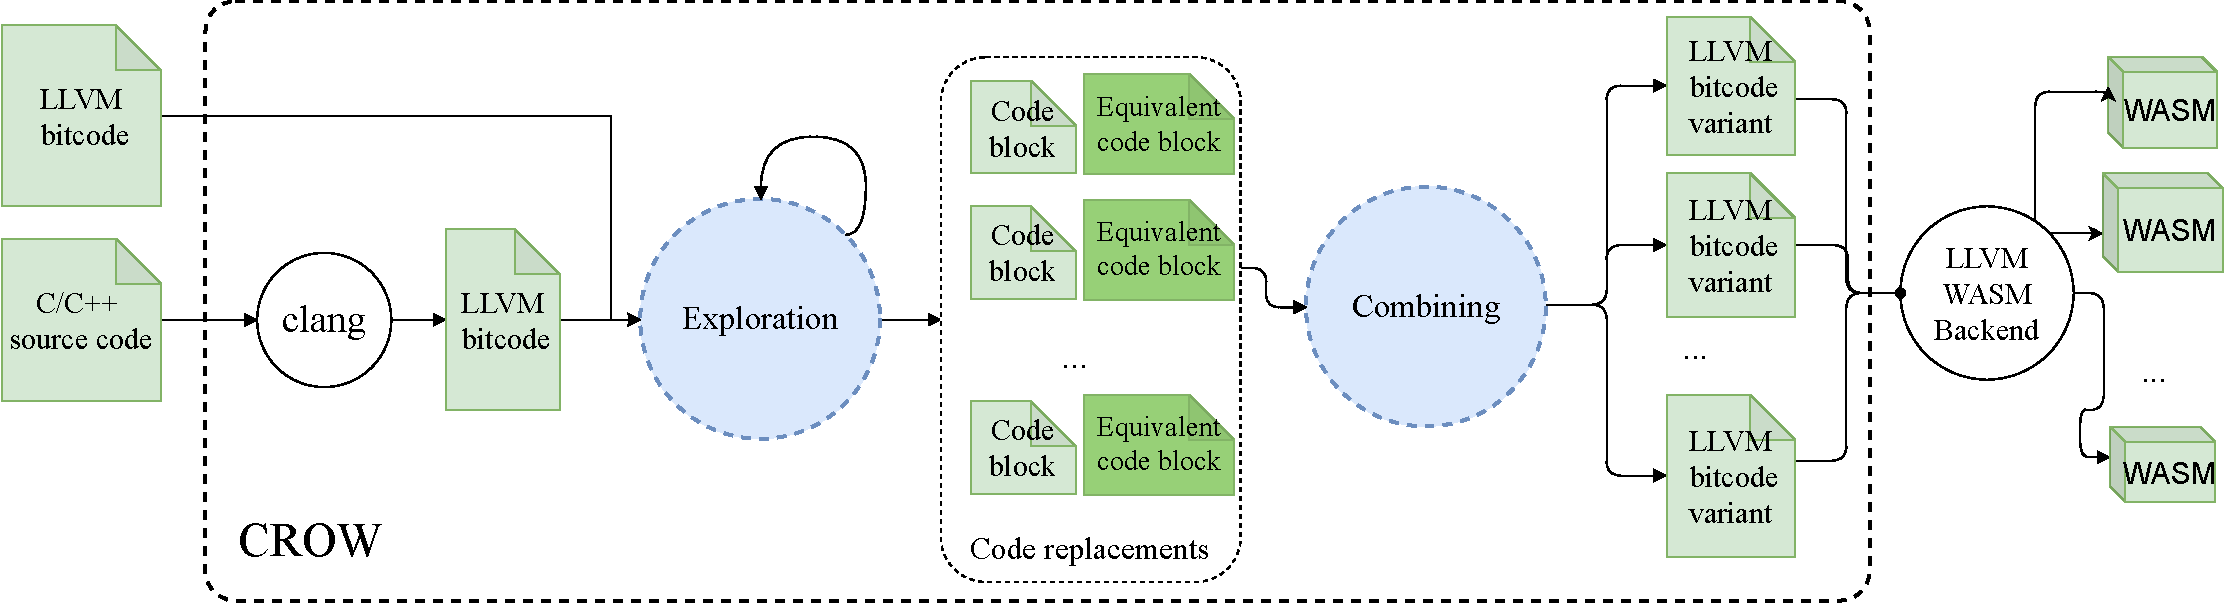
\includegraphics[width=\linewidth]{diagrams/generation/crow.drawio.pdf}
    \caption{CROW workflow to generate program variants. CROW takes C/C++ source codes or LLVM bitcodes to look for code blocks that can be replaced by semantically equivalent code and generates program variants by combining them.}
    \label{diagrams:crow}
\end{figure*}

Figure \ref{diagrams:crow} highlights the main two stages of the CROW's workflow, \textit{exploration} and \textit{combining}. The workflow starts by compiling the input program into the LLVM bitcode using clang from the source code. During the \emph{exploration} stage, CROW takes an LLVM bitcode and, for its code blocks, produces a collection of code replacements that are functionally equivalent to the original program. In the following, we enunciate the definitions we use along with this work for a code block, functional equivalence, and code replacement. 


\begin{definition}{Block (based on Aho \etal \cite{10.5555/6448}):}\label{def:code-block}
    Let $P$ be a program. A block $B$ is a grouping of declarations and statements in $P$ inside a function $F$. 
\end{definition}


\begin{definition}{Functional equivalence modulo program state (based on Le \etal \cite{10.1145/2594291.2594334}):}
    \label{def:functional-equivalence}
    Let $B_1$ and $B_2$ be two code blocks according to \autoref{def:code-block}. We consider the program state before the execution of the block, $S_i$, as the input and the program state after the execution of the block, $S_o$, as the output. $B_1$ and $B_2$ are functionally equivalent if given the same input $S_i$ both codes produce the same output $S_o$.
\end{definition}

\begin{definition}{Code replacement:}
    \label{def:code-replacement}
    Let $P$ be a program and $T$ a pair of code blocks $(B_1, B_2)$. $T$ is a candidate code replacement if $B_1$ and $B_2$ are both functionally equivalent as defined in \autoref{def:functional-equivalence}.
    Applying $T$ to $P$ means replacing $B_1$ by $B_2$. The application of $T$ to $P$ produces a program variant $P'$ which consequently is functionally equivalent to $P$.     
\end{definition}

We implement the \emph{exploration} stage by retargeting a superoptimizer for  LLVM, using its subset of the LLVM intermediate representation. CROW operates at the code block level, taking them from the functions defined inside the input LLVM bitcode module. In addition, the retargeted superoptimizer is in charge of finding the potential places in the original code blocks where a replacement can be applied. Finally, we use the enumerative synthesis strategy of the retargeted superoptimizer to generate code replacements.
The code replacements generated through synthesis are verified, according to \autoref{def:functional-equivalence}, by internally using a theorem prover. 

Moreover, we prevent the superoptimizer from synthesizing instructions that have no correspondence in \wasm for the sake of reducing the searching space for equivalent program variants. Besides, we disable all optimizations in the \wasm LLVM backend that could reverse the superoptimizer transformations, such as constant folding and instructions normalization.

%\todo{We disable cost restrictions and the LLVM backend optimizations...maybe for the assesment RQ ?}

In the \emph{combining} stage, CROW combines the candidate code replacements to generate different LLVM bitcode variants, selecting and merging the code replacements. 
Then for each combination, a variant bitcode is compiled into a \wasm binary if requested. Finally, CROW generates the variants from all possible combinations of code replacements as the power set of all code replacements.  

\end{comment}
%\chapter{Technical contributions/ Automatic Diversity for Wasm/ }
\label{chapter:technical}

\todo{Make a real introduction, the paragraphs below is too fast}

\todo{Create a new section from this, with a new figure as a high level architecture}


In the artifacts implemented with our contributions, we assume that the \wasm programs are generated through the LLVM compilation pipeline. This assumption is supported by the work of Hilbig et al. \cite{Hilbig2021AnES} in 2021 and the fact that LLVM-based compilers created the 70\% of \wasm binaries in the wild. Therefore,
our contributions diversify Wasm programs at the LLVM level. Other solutions would have been to diversify at the source code level, or at the \wasm binary level. However, the former would limit the applicability of our work. 
%Besides, as we discussed previously, our intention is also to study the impact of our contributions in edge computing and distributed systems and the top edge computing execution platforms, e.g. Cloudflare and Fastly, mostly take \wasm binaries as input. 
LLVM, on the contrary, supports different languages, with a rich ecosystem of frontends it it can reliably be retargeted to \wasm, thanks to the corresponding mature component in the LLVM toolchain. In addition, the LLVM ecosystem as a whole is very active, providing us with many different tools to facilitate our research endeavour.
In this chapter we summarize the technical details for our two contributions. \autoref{section:crow} we dissect the main components CROW \cite{CROW} implementation. Finally, in \autoref{section:mewe}, we describe the technical details of our second contribution, MEWE \cite{MEWE}.



\section{CROW}
\label{section:crow}

This section describes CROW \cite{CROW}, our first contribution. CROW is a tool tailored to create semantically equivalent \wasm variants out of a single program, either C/C++ and Rust code or LLVM bitcode.
In \autoref{diagrams:crow}, we describe the workflow of CROW to create program variants.
The figure highlights the main two stages of the CROW's workflow, \textit{exploration} and \textit{combining}. The workflow starts by compiling the input program into the LLVM bitcode using clang from the source code. During the \emph{exploration} stage, CROW takes an LLVM bitcode and, for its code blocks, produces a collection of code replacements that are functionally equivalent to the original program. 
%In the following, we enunciate the definitions we use along with this work for a code block, functional equivalence, and code replacement. 
In the \emph{combining} stage, CROW combines the code replacements to generate different LLVM bitcode variants. 
Then, a variant bitcode is compiled into a \wasm binary if requested. Finally, CROW generates the variants from all possible combinations of code replacements as the power set of all code replacements.  

%\subsection*{Overview}

\begin{figure*}[h]
    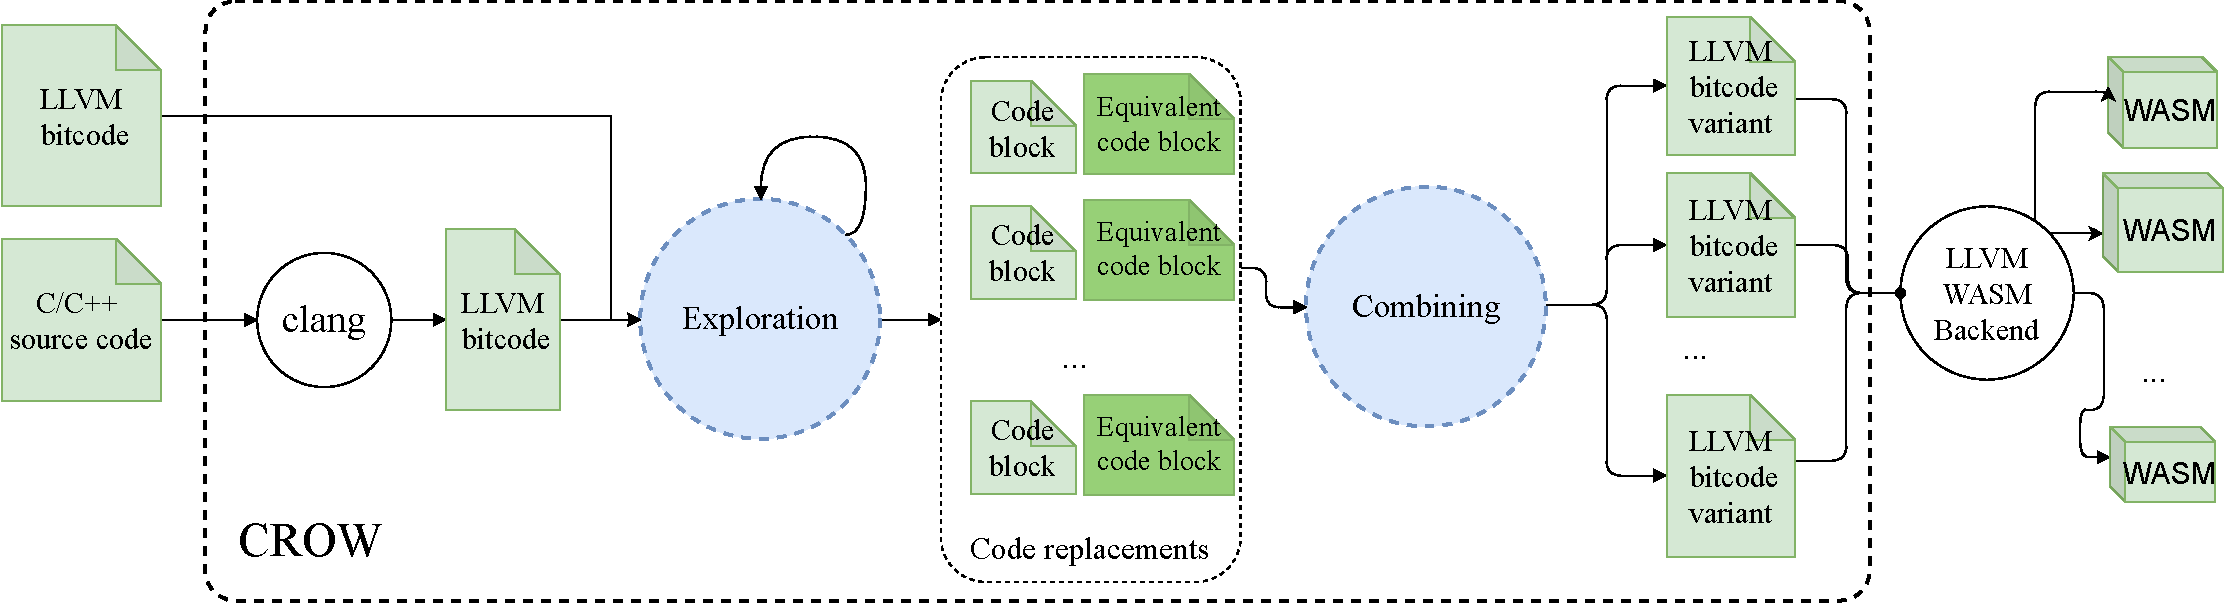
\includegraphics[width=\linewidth]{diagrams/generation/crow.drawio.pdf}
    \caption{CROW workflow to generate program variants. CROW takes C/C++ source codes or LLVM bitcodes to look for code blocks that can be replaced by semantically equivalent code and generates program variants by combining them.}
    \label{diagrams:crow}
\end{figure*}



%CROW operates at the code block level, taking them from the functions defined inside the input LLVM bitcode module. 
%In addition, the retargeted superoptimizer is in charge of finding the potential places in the original code blocks where a replacement can be applied. Finally, we use the enumerative synthesis strategy of the retargeted superoptimizer to generate code replacements.
%The code replacements generated through synthesis are verified, according to \autoref{def:functional-equivalence}, by internally using a theorem prover. 

\begin{comment}

\begin{definition}{Block (based on Aho \etal \cite{ahodragonbook}):}\label{def:code-block}
    Let $P$ be a program. A block $B$ is a grouping of declarations and statements in $P$ inside a function $F$. 
\end{definition}

\todo{Move to chapter 2}

\begin{definition}{Functional equivalence modulo program state (based on Cohen \etal \cite{cohen1993operating}):}
    \label{def:functional-equivalence}
    Let $B_1$ and $B_2$ be two code blocks according to \autoref{def:code-block}. We consider the program state before the execution of the block, $S_i$, as the input and the program state after the execution of the block, $S_o$, as the output. $B_1$ and $B_2$ are functionally equivalent if given the same input $S_i$ both codes produce the same output $S_o$.
\end{definition}

\begin{definition}{Code replacement:}
    \label{def:code-replacement}
    Let $P$ be a program and $T$ a pair of code blocks $(B_1, B_2)$. $T$ is a candidate code replacement if $B_1$ and $B_2$ are both functionally equivalent as defined in \autoref{def:functional-equivalence}.
    Applying $T$ to $P$ means replacing $B_1$ by $B_2$. The application of $T$ to $P$ produces a program variant $P'$ which consequently is functionally equivalent to $P$.     
\end{definition}
\end{comment}

\subsection*{Variants' generation}

CROW is based on the work of Jacob \etal \cite{jacob2008superdiversifier}. Their work uses code superoptimization to generate software diversification with an approach called superdiversification. 
% How a superoptimizer works
Code superoptimization focuses on \emph{searching} for a new program which is faster or smaller than the original code, while preserving its functionality.
The concept of superoptimizing a program dates back to 1987, with the seminal work of Massalin \cite{Massalin1987} which proposes an exhaustive exploration of the solution space. The search space is defined by choosing a subset of the machine's instruction set and generating combinations of optimized programs, sorted by length in ascending order. If any of these programs are found to perform the same function as the source program, the search halts. The main difference between the superoptimization process and a superdiversifier it that the latter keeps intermediate search results for the sake of diversification. 

We use the seminal work of Jacob and colleagues to implement CROW because of two main reasons.
First, the code replacements generated by this technique outperform diversification strategies based on hand-written rules. Besides, this technique is fully automatic.
Second, there is a battle tested superoptimizer for LLVM, Souper \cite{Sasnauskas2017Souper:Superoptimizer}. It dates from 2017 and has an active community of maintainers. By extending Souper with superdiversification, it allows us to contribute with a new mutation strategy, \emph{constant inferring} (in addition to the before mentioned strategies in \autoref{sota:sota}) to artificially generate diversification. We modify it to keep the intermediate solutions in their searching algorithm to generate program variants. Besides, 
we prevent Souper from synthesizing instructions that have no correspondence in the \wasm backend to reduce the searching space for variants. In addition, we disable the majority of the pruning strategies of Souper for the sake of more variants. Our modified version of Souper can be found at \todo{}.

% Souper
%Souper is an state-of-the-art superoptimizer for LLVM. It enumerates a set of several optimization candidates to be replaced.
%Souper is based on a Satisfiability Modulo Theories (SMT) solver. SMT solvers are useful for both verification and synthesis of programs \cite{10.1007/978-3-540-78800-3_24}.

%We implement the \emph{exploration} stage of CROW by retargeting Souper. The main objective of Souper is to find the best (smallest) possible program,  

\subsection*{Constant inferring}

As we previously mentioned, extending Souper as a superdiversifier contributes with a new mutation strategy called \emph{constant inferring}. 
The main component of Souper infers pieces of code as a single constant assignment particularly for boolean valued variables that are used to control branches.
If a program branching is removed due to a constant inferring, the generated program is considerably different to the original program, statically and dynamically.
Let us illustrate the case with an example.
The Babbage problem code is composed of a loop which stops when it discovers the smaller number that fits with the Babbage condition below.
\begin{center}
\begin{tabular}{c}

\lstset{language=C++,
                    style=CStyle,
                    basicstyle=\small\ttfamily,
                    columns=fullflexible,
                    breaklines=true, 
                    postbreak=\mbox{\textcolor{red}{$\hookrightarrow$}\space}}
\begin{lstlisting}[]
while((n * n) % 1000000 != 269696) n++;
\end{lstlisting}
\end{tabular}
\end{center}
% llvm-opt: rool unroll
In theory, this value can also be inferred by unrolling the loop the correct number of times with traditional tools like llvm-opt.
However, llvm-opt cannot unroll a \texttt{\textbf{while}}-loop because the loop count is too large.
% Souper
On the other hand, Souper can deal with this case, inferring the value of $n$ such that the Babbage condition is reached. Therefore, since the condition in the loop will always be false, the loop is dead code, and is removed in the final compilation. It is clear that the new program is remarkably different, smaller and faster than the original code.

When we retarget Souper we recombine all found replacements to create new programs, including those for which a constant inferring was performed.
This allows to create variants that are also better than the original program in terms of size and performance.

\subsection*{Removing latter optimizations for LLVM}

During the implementation of CROW we have the premise of removing all builtin optimizations in the LLVM compiler that could reverse Wasm variants.
Therefore, in addition to the extension of Souper, we modify the LLVM compiler and the \wasm backend.
We disable all optimizations in the \wasm backend that could reverse the superoptimizer transformations, such as constant folding and instructions normalization.


%\todo{We disable cost restrictions and the LLVM backend optimizations...maybe for the assesment RQ ?}

\subsection*{CROW instantiation}
%\label{section:crow:example}
%In \autoref{section:crow} we describe the main components and contributions of CROW. In this section we instantiate the workflow presented in \autoref{workflow} from the input of an example C code to the generation of a pool of \wasm program variants.

Let us illustrate how CROW works with the simple example code in \autoref{CExample}. The \texttt{f} function calculates the value of $2 * x + x$ where \texttt{x} is the input for the function.  CROW compiles this source code and generates the intermediate LLVM bitcode in the left most part of \autoref{example:crow:original:llvm}. CROW potentially finds two code blocks to look for variants, as the right-most part of \autoref{example:crow:original:llvm} shows.

% snippet of code showing the detection of code blocks
    
\begin{code}
    \lstset{language=C,
    basicstyle=\small\ttfamily,caption={C function that calculates the quantity $2x + x$},label=CExample}
    \begin{lstlisting}[style=CStyle]
int f(int x) { 
    return 2 * x + x; 
}    
    \end{lstlisting}
    
\end{code}

\lstdefinelanguage{LLVM}
    {morekeywords={i32,mul,align,nsw,add,load,store,define,br, ret, shl, ret},
    sensitive=false,
    morecomment=[l]{;},
    morecomment=[s]{;}{;},
    morestring=[b],
}
\lstdefinestyle{nccode}{
    numbers=left,
    tabsize=4,
    showspaces=false,
    breaklines=true, 
    showstringspaces=false,
    moredelim=**[is][{\btHL[fill=black!10]}]{`}{`},
    moredelim=**[is][{\btHL[fill=celadon!40]}]{!}{!}
}
\lstset{
    language=LLVM,
    style=nccode,
    %basicstyle=\small\ttfamily,
    columns=fullflexible,
    breaklines=true
}


\begin{code}
    \centering
    \captionof{lstlisting}{LLVM's intermediate representation program, its extracted instructions and replacement candidates. Gray highlighted lines represent original code, green for code replacements. }\label{example:crow:original:llvm}
    \lstset{numbers=none}
    \noindent\begin{minipage}[t]{.33\linewidth}
    \centering
    \begin{lstlisting}[xleftmargin=1em,escapechar=?]
    define i32 @f(i32) {

    ?\tikzmarkWS{2}{code 2}{11.5}{10}{3.5cm}?
    ?\tikzmarkWS{1}{code 1}{11.5}{3.5}{3.0cm}?
    %2 = mul nsw i32 %0,2
    %3 = add nsw i32 %0,%2 

    ret i32 %3
    }
    
    define i32 @main() {
    %1 = tail call i32 @f(i32 10)
    ret i32 %1
    }
    \end{lstlisting}
    \end{minipage}%\hfill%
    \begin{minipage}[t]{.32\linewidth}
        \begin{lstlisting}[xleftmargin=1em,escapechar=?]
?Replacement candidates for code\_1?

`%2 = mul nsw i32 %0,2`

!%2 = add nsw i32 %0,%0!

!%2 = shl nsw i32 %0, 1:i32!
    \end{lstlisting}
    \end{minipage}%\hfill%
    \begin{minipage}[t]{.32\linewidth}
        \lstdefinestyle{nccode}{
        tabsize=4, 
        showspaces=false,
        breaklines=true, 
        showstringspaces=false,
        moredelim=**[is][{\btHL[fill=black!10]}]{`}{`},
        moredelim=**[is][{\btHL[fill=celadon!40]}]{!}{!}
        }
        \lstset{
            language=LLVM,
            style=nccode,
            columns=fullflexible,
            breaklines=true,
            belowcaptionskip=1pt,
            abovecaptionskip=1pt,
        } 
        \begin{lstlisting}[name={B},escapechar=?]
?Replacement candidates for code\_2?

`%3 = add nsw i32 %0,%2`

!%3 = mul nsw %0, 3:i32!
        \end{lstlisting}
    \end{minipage}
    
\end{code}





\begin{code}
    \centering
    \captionof{lstlisting}{Candidate code replacements combination. Orange highlighted code illustrate replacement candidate overlapping.}\label{example:crow:original:combination}
    \lstset{numbers=none}
    \noindent\begin{minipage}[t]{.5\linewidth}
    \begin{lstlisting}[xleftmargin=1em,escapechar=?]
`%2 = mul nsw i32 %0,2`
`%3 = add nsw i32 %0,%2`

!%2 = add nsw i32 %0,%0!
`%3 = add nsw i32 %0,%2`

!%2 = shl nsw i32 %0, 1:i32!
`%3 = add nsw i32 %0,%2`

    \end{lstlisting}
    \end{minipage}%\hfill%
    \begin{minipage}[t]{.5\linewidth}
        \lstdefinestyle{nccode}{
        tabsize=4, 
        showspaces=false,
        breaklines=true, 
        showstringspaces=false,
        moredelim=**[is][{\btHL[fill=black!10]}]{`}{`},
        moredelim=**[is][{\btHL[fill=celadon!40]}]{!}{!},
        moredelim=**[is][{\btHL[fill=weborange!40]}]{'}{'}
        }
        \lstset{
            language=LLVM,
            style=nccode,
            columns=fullflexible,
            breaklines=true,
            belowcaptionskip=1pt,
            abovecaptionskip=1pt,
        } 
        \begin{lstlisting}[xleftmargin=1em,escapechar=?]
'%2 = mul nsw i32 %0,2'
!%3 = mul nsw %0, 3:i32!

'%2 = add nsw i32 %0,%0'
!%3 = mul nsw %0, 3:i32!

'%2 = shl nsw i32 %0, 1:i32'
!%3 = mul nsw %0, 3:i32!

    \end{lstlisting}
    \end{minipage}
\end{code}


\begin{tikzpicture}[remember picture,overlay]
%\path (2.north) edge[<-, bend left] (1.north);
%\path[draw, ->] (3.west) edge[<-, bend left] (2.west);
%\path (4.west) edge[<-, bend left] (3.west);
%\path (1.south) edge[<-, bend left] (4.south);

%\path (2.east) edge[<-, bend left, blue] (5.north);
%\path (3.east) edge[<-, bend right, olive] (2.east);
%\path (1.east) edge[<-, bend left, black] (replall1.west);
%\path (2.east) edge[<-, bend left, black] (replall2.west);
%\path (rep11.east) edge[<-, bend left, black] (6.east);
%\path (9.east) edge[<-, bend right, black] (4.east);
%\path (7.east) edge[<-, bend right, black] (8.east);
%\path (5.south) edge[<-, bend right, blue] (4.east);
%\path (9.north) edge[<-] (8.south);
%\path (5.south) edge[<-, bend left] (9.south);


%\path (10.north) edge[<-, bend left] (11.north);
%\path (11.south) edge[<-, bend left] (10.south);
%\path (7) edge[<-, bend right] (6.east);
%\path (8) edge[<-, bend right] (7.east);
\end{tikzpicture}


    

CROW, in the exploration stage detects 2 code blocks, \texttt{code\_block\_1} and \texttt{code\_block\_2} as the enclosing boxes in the left most part of \autoref{example:crow:original:llvm} shows. CROW synthesizes $2 + 1$ candidate code replacements for each code block respectively as the green highlighted lines show in the right most parts of \autoref{example:crow:original:llvm}.
The baseline strategy of CROW is to generate variants out of all possible combinations of the candidate code replacements, \ie uses the power set of all candidate code replacements.

In the example, the power set is the cartesian product of the found candidate code replacements for each code block, including the original ones, as \autoref{example:crow:original:combination} shows. The power set size results in $6$ potential function variants. Yet, the generation stage would eventually generate $4$ variants from the original program. CROW generated 4 statically different Wasm files, as \autoref{example:crow:variants:wasm} illustrates. This gap between the potential and the actual number of variants is a consequence of the redundancy among the bitcode variants when composed into one. In other words, if the replaced code removes other code blocks, all possible combinations having it will be in the end the same program. In the example case, replacing \texttt{code\_block\_2} by \texttt{mul nsw \%0, 3}, turns \texttt{code\_block\_1} into dead code, thus, later replacements generate the same program variants. The rightmost part of \autoref{example:crow:original:combination} illustrates how for three different combinations, CROW produces the same variant. We call this phenomenon a candidate code replacement overlapping.

One might think that a reasonable heuristic could be implemented to avoid such overlapping cases. Instead, we have found it easier and faster to generate the variants with the combination of the replacement and check their uniqueness after the program variant is compiled. This prevents us from having an expensive checking for overlapping inside the CROW code. Still, this phenomenon calls for later optimizations in future works.

\lstdefinestyle{nccode}{
        numbers=none,
        firstnumber=2,
        stepnumber=1,
        numbersep=10pt,
        tabsize=4, 
        showspaces=false,
        breaklines=true, 
        showstringspaces=false,
    moredelim=**[is][\btHL]{`}{`},
    moredelim=**[is][{\btHL[fill=black!10]}]{`}{`},
    moredelim=**[is][{\btHL[fill=celadon!40]}]{!}{!}
}

\lstset{
    language=WAT,
    style=nccode,
    basicstyle=\footnotesize\ttfamily,
    columns=fullflexible,
    breaklines=true
}


\begin{code}
    \centering
    \captionof{lstlisting}{\termidx{Wasm }program variants generated from program \autoref{CExample}.}\label{example:crow:variants:wasm}
    \lstset{numbers=none}
    \noindent\begin{minipage}[t]{.45\linewidth}
    \begin{lstlisting}[xleftmargin=1em,escapechar=?]
func $f (param i32) (result i32)
   local.get 0
    `i32.const 2`
    `i32.mul`
    `local.get 0`
    `i32.add`

        \end{lstlisting}
\begin{lstlisting}[xleftmargin=1em,escapechar=?]
func $f (param i32) (result i32)
    local.get 0
    !local.get 0!
    !i32.add!
    `local.get 0`
    `i32.add`

                \end{lstlisting}
    \end{minipage}\hfill
    \noindent\begin{minipage}[t]{.45\linewidth}
\begin{lstlisting}[xleftmargin=1em,escapechar=?]
func $f (param i32) (result i32)
    local.get 0
    !i32.const 1!
    !i32.shl!
    `local.get 0`
    `i32.add`

    \end{lstlisting}
\begin{lstlisting}[xleftmargin=1em,escapechar=?]
func $f (param i32) (result i32)
    local.get 0
    !i32.const 3!
    !i32.mul!

            \end{lstlisting}
        \end{minipage}
\end{code}





\section{MEWE: Multi-variant Execution for WEbAssembly}
\label{section:mewe}

\newcommand{\tool}{MEWE\xspace}
\newcommand{\repourl}{TODO}
% Overview
This section describes MEWE \cite{MEWE}, our second contribution. 
%MEWE is implemented in 942 lines of C++ code.
The core idea of \tool is to synthesize diversified function variants, using CROW, providing execution-path randomization in an MVE.
The tool generates application-level multivariant binaries, without any change to the operating system or \wasm runtime.
%It uses the LLVM 12.0.0 libraries to extend the LLVM standard linker tool capability with the multivariant generation.
%Per Crane et al. the execution-path randomization is made to hinder side-channel attacks \cite{crane2015thwarting}. 
% All programs are diversified with behavior preservation guarantees according to the design of CROW (\autoref{section:crow}).
MEWE creates an MVE by intermixing functions for which CROW generates variants, as step \step{2} in \autoref{diagrams:generic} shows.
CROW generates each one of these variants with fine-grained diversification at instruction level, applying the majority of the strategies discussed in \autoref{sota:sota} and \emph{constant inferring}. Besides, \tool inlines function variants when appropriate, also resulting in call stack diversification at runtime.

In \autoref{workflow} we zoom MEWE(\step{4}) from the diagram in \autoref{diagrams:generic}. MEWE takes the LLVM IR variants generated by our diversifier and merges them into a Wasm multivariant.
In the figure, we highlight the two components of MEWE. 
In Step~\step{I}, we merge the LLVM IR variants created by CROW and we create a LLVM multivariant binary.
In Step~\step{II}, we use a special component, called a ``Mixer``,  which augments the binary with a random generator, which is required for performing the execution-path randomization. 
Also at this stage, the multivariant binary is fixed with the entrypoint of the original binary.
%The harness is used to connect the program to its original execution environment while the generator provides support for random execution path at runtime.
The final output of Step~\step{III} is a standalone multivariant \wasm binary that can be directly deployed. 
%For sake of open science and for fostering research on this important topic, the code of \tool is made publicly available on GitHub: \repourl.

\begin{figure*}
  \centering
  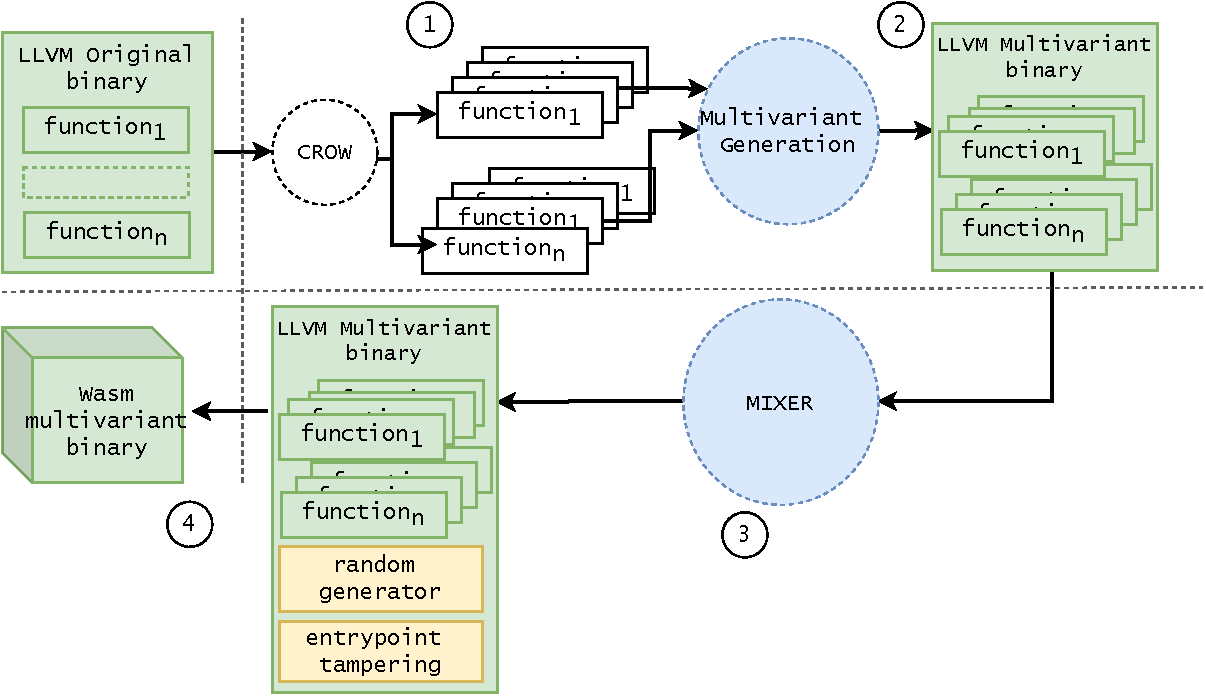
\includegraphics[height=3.1in]{diagrams/MEWE.pdf}
  \caption{Overview of \tool. It takes as input an LLVM binary. It first generates a set of functionally equivalent variants for each function in the binary and then generates a LLVM multivariant binary composed of all the function variants. Also, it includes the dispatcher functions in charge of selecting a variant when a function is invoked. The \tool mixer composes the LLVM multivariant binary with a random number generation library and a tampering of the original application entrypoint, in order to produce a \wasm multivariant binary ready to be deployed. }
  \label{workflow}
\end{figure*}


\subsection*{Multivariant generation}

The key component of \tool consists in combining the variants into a single binary.
The goal is to support execution-path randomization at runtime.
% General idea
The core idea is to introduce one dispatcher function per original function with variants.
A dispatcher function is a synthetic function that is in charge of choosing a variant at random, every time the original function is invoked during the execution.
With the introduction of dispatcher function,  \tool turns the original call graph into a multivariant call graph, defined as follows. 

\begin{definition}{Multivariant Call Graph (MCG):}\label{def:EP}
  
    A multivariant call graph is a call graph $\langle N,E \rangle$ where the nodes in $N$ represent all the functions in the binary and an edge $(f_1,f_2) \in E$ represents a possible invocation of $f_2$ by $f_1$  \cite{ryder1979}, where the nodes are typed. The nodes in $N$ have three possible types: a function present in the original program,  a generated function variant, or a dispatcher function.
\end{definition}


\begin{figure}
    \centering
  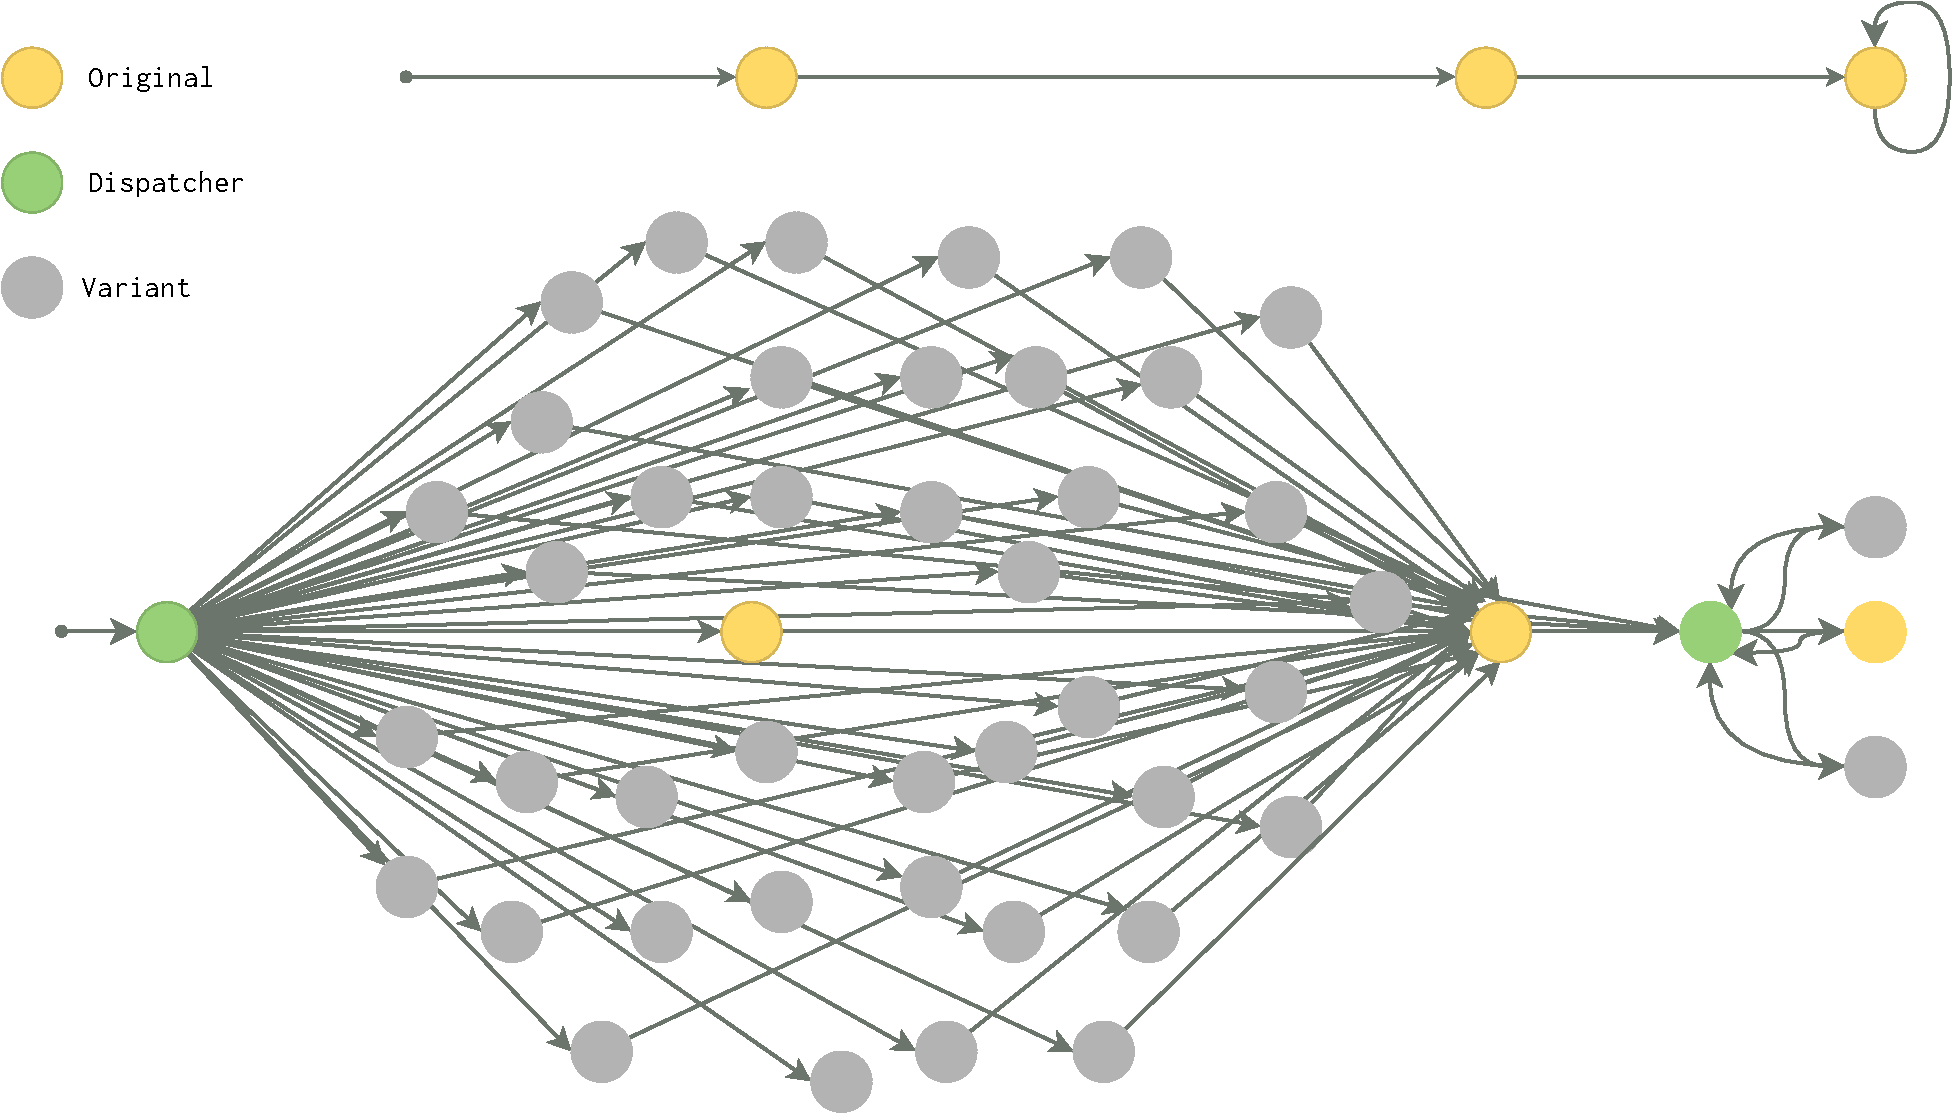
\includegraphics[width=.8\linewidth]{diagrams/CFG.pdf}
  \caption{Example of two static call graphs. At the top, the original call graph, at the bottom, the multivariant call graph, which includes nodes that represent function variants (in grey), dispatchers (in green), and original functions  (in yellow).
}
  \label{multivariant}
\end{figure}

% Instance of a multivariant module
In \autoref{multivariant}, we show the original static call graph for and original program (top of the figure), as well as the multivariant call graph generated with \tool (bottom of the figure).
The grey nodes represent function variants, the green nodes function dispatchers and the yellow nodes are the original functions.
The possible calls are represented by the directed edges.
The original program includes 3 functions. \tool generates 43 variants for the first function, none for the second and three for the third function. 
\tool introduces two dispatcher nodes, for the first and third functions. Each dispatcher is connected to the corresponding function variants, in order to invoke one variant randomly at runtime.


% exaplanation of dispatcher
In  \autoref{listing:multivariant_template}, we illustrate the LLVM construction for the function dispatcher corresponding to the right most green node of \autoref{multivariant}.
% General logic of a multivartiant function
It first calls the random generator, which returns a value that is then used to invoke a specific function variant. 
% Why a linear based switch
We implement the dispatchers with a switch-case structure to avoid indirect calls that can be susceptible to speculative execution based attacks \cite{Narayan2021Swivel}. 
The choice of a switch-case also avoids having multiple function definitions with the same signature, which could increase the attack surface in case the function signature is vulnerable \cite{johnson2021}.
This also allows \tool to inline function variants inside the dispatcher, instead of defining them again.
Here we trade security over performance, since dispatcher functions  that perform indirect calls, instead of a switch-case,  could improve the performance  of the dispatchers as indirect calls have constant time.
%It should be noted that the dispatcher function is constructed using the same signature as the original function. 


\lstset{
    language=llvm,
    %style=nccode,
    basicstyle=\footnotesize\ttfamily,
    columns=fullflexible,
    breaklines=true,
    numbers=none,
    stepnumber=1,
    float
}

\begin{code}
\scriptsize
\noindent\begin{minipage}[b]{\linewidth}
    \begin{minipage}[t]{1\linewidth}
        \begin{lstlisting}[escapeinside={(*}{*)}]
define internal i32 @foo(i32 %0) {
    entry:
      %1 = call i32 @discriminate(i32 3)
      switch i32 %1, label %end [
        i32 0, label %case_43_
        i32 1, label %case_44_
      ]
    case_43_:                 
      %2 = call i32 @foo_43_(%0)
      ret i32 %2
    case_44_:                
      %3 = <body of foo_44_ inlined>
      ret i32 %3
    end:                                             
      %4 = call i32 @foo_original(%0)
      ret i32 %4
}
        \end{lstlisting}
    \end{minipage}%
    
    \noindent\rule{\linewidth}{0.4pt}
    \captionof{lstlisting}{Dispatcher function embedded in the multivariant binary of the original function in the rightmost green node in \autoref{multivariant}.}\label{listing:multivariant_template}
\end{minipage}
\end{code}

\subsection*{Mixer}

The Mixer has four specific objectives: tamper the entrypoint of the application, link the LLVM multivariant binary, inject a random generator and merge all these components into a multivariant \wasm binary.
% Implementation
We use the Rustc compiler\footnote{\url{https://doc.rust-lang.org/rustc/what-is-rustc.html}} to orchestrate the mixing.
% The random number generation
For the random generator, we rely on WASI's specification \cite{WASI} for the random behavior of the dispatchers. Its exact implementation is dependent on the platform on which the binary is deployed.

The \tool mixer creates a new entrypoint for the binary called \emph{entrypoint tampering}.
It simply wraps the dispatcher for the entrypoint variants as a new function for the final Wasm  binary and is declared as the application entrypoint. %This fixes an issue with  

% How to turn function into endpoints
%The entrypoint tampering is needed for binariess passed to MEWE. We refer to the entrypoint as the entering main function of the original binary passed to MEWE. The tampering is needed because dispatchers for entrypoint variants make the multivariant invalid to be directly executed after it is compiled to Wasm.

%Throughout this paper, we refer to an endpoint as the closure of invoked functions when the entry point of the \wasm binary is executed.



\begin{comment}

\subsection{Multivariant Binary Execution at the Edge}

\todo{Introduce as the use of MEWE}

% What really is executed is the x86 code
When a WebAssembly binary is deployed on an edge platform, it is translated to machine code on the fly.
For our experiment, we deploy on the production edge nodes of Fastly. This edge computing platform uses Lucet, a native WebAssembly compiler and runtime, to compile and run the deployed Wasm  binary \footnote{\url{https://github.com/bytecodealliance/lucet}}.
Lucet generates x86 machine code and ensures that the generated machine code executes inside a secure sandbox, controlling memory isolation.


\begin{figure}
\centering
  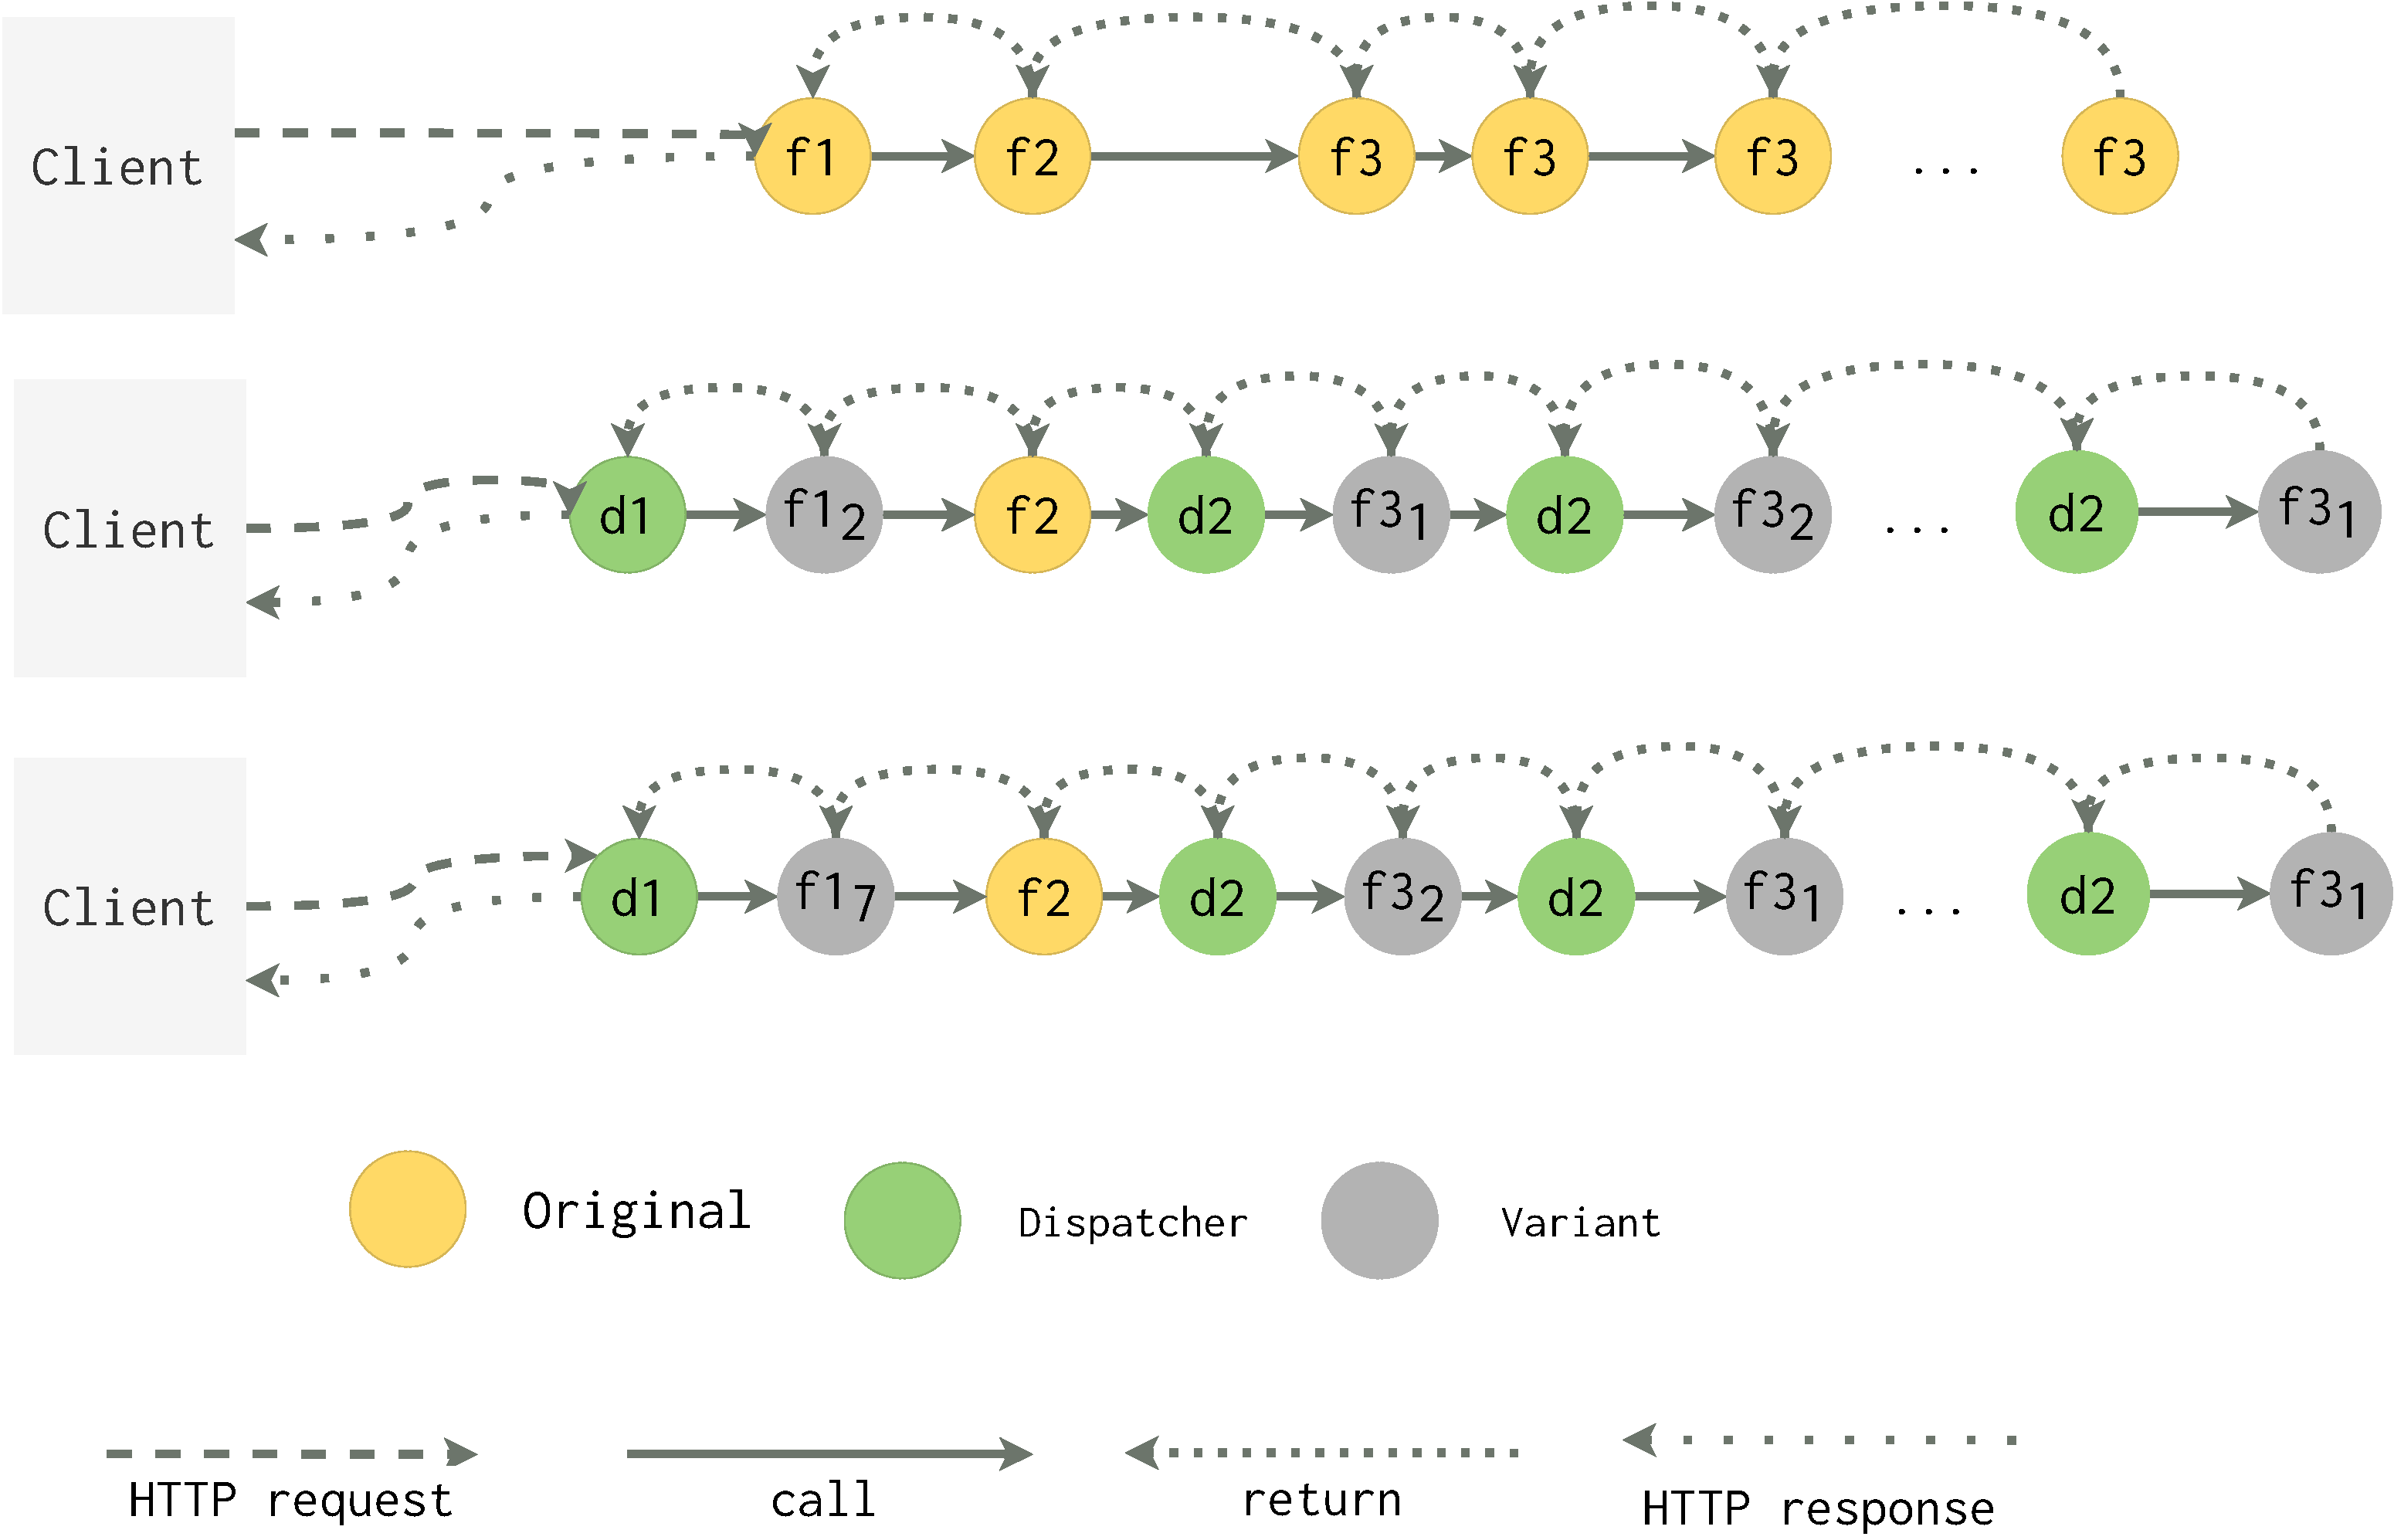
\includegraphics[width=1\linewidth]{diagrams/traces.pdf}
  \caption{Top: an execution trace for the  \texttt{bin2base64} endpoint. Middle and bottom: two different execution traces for the multivariant \texttt{bin2base64}, exhibited by two different requests with exactly the same input.}
  \label{http:workflow}
\end{figure}

% How it works
\autoref{http:workflow} illustrates  the runtime behavior of the original and the multivariant binary,  when deployed on an Edge node.
The top most diagram illustrates the execution trace for the  original of the endpoint \texttt{bin2base64}.
When the HTTP request with the input \texttt{"Hello World!"} is received, it invokes functions $f1$, $f2$ followed by 27 recursive calls of function $f3$. Then, the endpoint sends the result \texttt{"0x000xccv0x10x00b3Jsx130x000x00 0x00xpopAHRvdGE="} of its base64 encoding in an HTTP response.

The two diagrams at the bottom of \autoref{http:workflow} illustrate two executions traces observed through two different requests to the endpoint \texttt{bin2base64}.
In the first case, the request first triggers the invocation of dispatcher $d1$, which randomly decides to invoke the variant $f1_2$; then $f2$, which has not been diversified by \tool, is invoked; then the recursive invocations to $f3$ are replaced by iterations over the execution of dispatcher $d2$ followed by a random choice of variants of $f3$. Eventually the result is computed and sent back as an HTTP response. 
The second execution trace of the multivariant binary shows the same sequence of dispatcher and function calls as the previous trace, and also shows that for a different requests, the variants of $f1$ and $f3$ are different. 


The key insights from these figures are as follows. First, from a client's point of view, a request to the original or to a multivariant endpoint, is completely transparent. Clients send the same data, receive the same result, through the same protocol, in both cases.
Second, this figure shows that, at runtime, the execution paths for the same endpoint are different from one execution to another, and that this randomization process results from multiple random choices among function variants, made through the execution of the endpoint.
%From an attacker's perspective, this random selection of variants constantly moves the attack surface and is meant to render a potential vulnerability harder to reach or exploit \cite{davi2015isomeron, 10.5555/3091125.3091155, BEKIROGLU2021106601}.


\end{comment}




\section*{Conclusions}

This chapter discusses the technical details for the artifacts implemented for our two contributions.
We describe how CROW generates program variants.
We introduce a new mutation strategy that is a consequence of retargeting a superoptimizer for LLVM as a superdiversifier.
Besides, we dissect MEWE and how it creates an MVE system.
In \autoref{chapter:method} we discuss the methodology we follow to evaluate the impact of CROW and MEWE.
%\chapter{Methodology} 
\label{chapter:method}

\pagestyle{plain}
% Define some numbers here for the autmation of the tables
\newcommand{\libsodiumfunctions}{869}
\newcommand{\qrcodefunctions}{1849}
\newcommand{\allmewefunctions}{\libsodiumfunctions + \qrcodefunctions}

% Execute a python script for small calculations
\newcommand{\py}[1]{\input{|python3 interpreter.py #1}}
\newcommand{\fromjson}[2]{\input{| jq -r '#2' '#1}}

\newcommand{\corpusrosetta}{Rosetta\xspace}
\newcommand{\corpussodium}{Libsodium\xspace}
\newcommand{\corpusqrcode}{QrCode\xspace}


\newcommand{\DTWStatic}{dt\_static\xspace}
\newcommand{\DTW}{TraceDiff\xspace}
\renewcommand{\tool}{CROW\xspace}

%\todo{Recheck the selection of the modules for sodium}

%This chapter investigates whether we can artificially create program variants through semantically equivalent code transformations. We propose a framework to generate program variants functionally equivalent to their original.
%We introduce the retargeting of a superoptimizer, using its exhaustive search strategy to provide semantically equivalent code transformations. 
%The presented methodology and transformation tool, CROW, are contributions to this thesis.
%We evaluate the usage of CROW on two corpora of open-source and nature diverse programs. 
In this chapter, we present our methodology to answer the research questions enunciated in \autoref{intro:definition:rq}.
We investigate three research questions. In the first question, we aim to investigate the static differences between variants. We evaluate the code properties the lead less or more software diversification.
Our second research question focuses on comparing their behavior during their execution, complementing our first research question. The generated variants should be statically different, but also should provide different observable behavior. 
The final research question evaluates the feasibility of using the program variants in security-sensitive environments. We evaluate our generated program variants in an Edge-Cloud computing platform proposing a novel multivariant execution approach.

% \todo{too generic: READ AGAIN to see how to land this
The main objective of this thesis is to study the feasibility of automatically creating program variants out of preexisting program sources. To achieve this objective,
we use the empirical method \cite{Runeson2020}, proposing a solution and evaluating it through quantitative analyzes in case studies. We follow an iterative and incremental approach on the selection of programs for our corpora. To build our corpora, we find a representative and diverse set of programs to generalize, even when it is unrealistic following an empirical approach, as much as possible our results.
We first enunciate the corpora we share along this work to answer our research questions. Then, we establish the metrics for each research question, set the configuration for the experiments, and describe the protocol.

% Our approach lies under \textit{Design Science} \cite{Runeson2020}, in terms of empirical validation, the scope of the design knowledge gained in a study can be extended by systematically extending the scope of the valudation in subsequent studies. Thus, the size of our corpora can be extended to increase the knowledge of the research area.


\section{Corpora}
\label{section:crow:corpora}

Our experiments assess the impact of artificially created diversity. The first step is to build a suitable corpus of programs' seeds to generate the variants. Then, we answer all our research questions with three corpora which follow two main properties: 1) \emph{functionally diverse:} the selection of the programs is not biased by functionally fixed tasks, for example, the programs in one of our corpora solve from the \textit{Babbage} problem to \textit{Convex Hull} calculation; and 2) \emph{representative:} our corpora have 3021 programs that can be ported to \wasm, representing approximately 40\% of the unique Wasm binaries in the wild \cite{Hilbig2021AnES}.


We build our three corpora in an escalating strategy based on the merging of our previous publications. The first corpus is diverse and contains simple programs in terms of code size, making them easy to manually analyze. The second corpus is a project meant for security-sensitive applications. The third corpus is a QR encoding decoding algorithm. 
%The work of Hilbig \etal \cite{Hilbig2021AnES} shows that approximately 65\% of all \wasm programs come out of C/C++ source code through the LLVM pipeline, and more than 75\% if the Rust language is included. Therefore, all modules in the corpora are considered to come along the LLVM pipeline. 
In the following, we describe the filtering and description of each corpus.

\begin{enumerate}
    \item \textbf{\corpusrosetta}: We take programs from the Rosetta Code project\footnote{\url{http://www.rosettacode.org/wiki/Rosetta_Code}}. This website hosts a curated set of solutions for specific programming tasks in various programming languages. It contains many tasks, from simple ones, such as adding two numbers, to complex algorithms like a compiler lexer. We first collect all C programs from the Rosetta Code, representing $989$ programs as of 01/26/2020. We then apply several filters: the programs should successfully compile and, they should not require user inputs to automatically execute them, the programs should terminate and should not result in non-deterministic results. 
    
    The result of the filtering is a corpus of 303 C programs. All programs include a single function in terms of source code. These programs range from $7$ to $150$ lines of code.

    \item \textbf{\corpussodium}: This project is encryption, decryption, signature, and password hashing library implemented in 102 separated modules. The modules have between $8$ and $2703$ lines of code per function. This project is selected based on two main criteria: first, its importance for security-related applications, and second, its suitability to collect the modules in LLVM intermediate representation. %We select 5 programs that interconnect the 102 modules of the project.

    \item \textbf{\corpusqrcode}: This project is a QrCode and MicroQrCode generator written in Rust. This project contains 2 modules having between $4$ and $725$ lines of code per function. As \corpussodium, we select this project due to its suitability for collecting the modules in their LLVM representation. Remarkably, this project increases the complexity of the previously selected projects due to its integration with the generation of images.
    
\end{enumerate}

In \autoref{table:corpora} we listed the corpus name, the language of the programs in the corpus, the number of modules, the total number of functions, the range of lines of code, and the original location of the corpus. 


%The first corpus, \textbf{CROW prime}, . The second corpus, \textbf{MEWE prime}, is part of the MEWE contribution \cite{}. In \autoref{table:corpora} we summarize the selection criteria, and we mention each corpus properties. With both corpora we evaluate CROW with a total of $303 + \py{\allmewefunctions}$ functions. 

\begin{table}[h]
    \renewcommand{\arraystretch}{1.0}
    \small
    \centering
    \begin{tabular}{l | p{1cm} | l | l | l | p{3.2cm}}
        Corpus & Lang. & No. modules & No. functions & LOC range & Location \\
        \midrule
            % CROW
            \corpusrosetta & C &
            - %\footnote{ The concept of module does not apply for this corpus programs. } 
            &
            303  & 
            7 - 
            150 & 
            \url{https://github.com/KTH/slumps/tree/master/benchmark_programs/rossetta/valid/no_input}\\
        \hline
        \corpussodium & LLVM IR + Rust &
        102 &
        869  &
        8 - 2703 &   
        \url{https://github.com/jedisct1/libsodium/tree/2b5f8f2b6810121c2d9a8cc8a392e01f4d3de433 }\\
        \hline
        \corpusqrcode & LLVM IR + Rust &
        2 &
        1849  & 
        4 - 725   & 
        \url{https://github.com/kennytm/qrcode-rust/commit/faa4397ba7c5f441cb9a2b436c1e84a0d52ae942} \\
        % Total stats
        \hline
        \hline
        \textbf{Total} & & 
        & 
        \py{ 303 + \qrcodefunctions + \libsodiumfunctions} &  
        &     \\

    \end{tabular}
    \caption{Corpora description. The table is composed by the name of the corpus, programming language of the programs in the corpus, the number of modules, the number of functions, the lines of code range and the location of the corpus.}
    \label{table:corpora}
\end{table}


\section{\rqone}
\label{rq1:method}

\begin{figure}[h]
    \centering
    \includegraphics[height=4.1in]{diagrams/RQ1.pdf}
    \caption{The program variants generation for RQ1.}
    \label{diagrams:protocol:rq1}
\end{figure}


This research question investigates whether we can artificially generate program variants for \wasm. We use CROW to generate variants from an original program, written in C/C++ in the case of the \corpusrosetta corpus and LLVM bitcode modules in the case of the \corpussodium and \corpusqrcode. 
In \autoref{diagrams:protocol:rq1} we illustrate the workflow to generate \wasm\ program variants. We pass each function of the corpora to CROW as a program to diversify. To answer RQ1, we study the outcome of this pipeline, the generated \wasm\ variants. 


\subsection*{Metrics}

To assess our approach's ability to generate \wasm\ binaries that are statically different, we compute the number of variants and the number of unique variants for each original function of each corpus. 
On top, we define the aggregation of these former two values to quantitatively evaluate RQ1 at the corpus level. 

We start by defining what a program's population is. This definition can be applied in general to any collection of variants of the same program. All definitions are based upon bytecodes and not the source code of the programs.

\begin{definition}{Program's population $M(P)$:}\label{def:rq1:programspopulation}
    \normalfont 
    Given a program P and its generated variants $v_i$, the program's population is defined as:\\
    $$
        M(P)=\{v_i\ \text{where $v_i$ is a variant of P}\}
    $$

    Notice that the program's population includes the original program P.
\end{definition}

Beyond the program's population, we also want to compare how many program variants are unique. The subset of unique programs in the program's population hints how the variants are different between them and not only against the original program. For example, imagine a program $P$ with two program variants $V_1$ and $V_2$, the program population is composed by $\{P, V_1 \text{ and } V_2\}$, where $V_1$ is different from $P$, and $V_2$ is different from $P$. $V_1$ is either equal or different from $V_2$, the program's population still be the same. If $V_1$ and $V_2$ are equal, then only one unique variant is generated,

%\todo{
%   clarify source code versus byte code for earch definition.

%why are those definitions important? interesting? why do you introduce them?
%}
%Notice that all metrics over programs and their variants make sense only at the population level. Therefore, we compare semantically equivalent programs from the same population.

%\todo{
%   difference unclear or trivial.

%do you need source code versus bytecode?

%clarify
%}

\begin{definition}{Program's unique population $U(P)$:}\label{def:rq1:programsuniquepopulation}
    \normalfont 
    Given a program P and its program's population $M(P)$, the program's unique population is defined as.\\
    $$
        U(P)=\{v\ \in\ M(P)\}
    $$
    such that $\forall v_i,v_j \in U(P)$, $v_i \neg v_j$ $\Rightarrow$ $md5sum(v_i) \ne md5sum(v_j)$.
    $Md5sum(v)$ is the md5 hash calculated over the bytecode stream of the program file $v$. Notice that the original program $P$ is included in $U(P)$.

\end{definition}

\begin{metric}{Program's population size $S(P)$:}\label{metric:rq1:PS}
    \normalfont 
    Given a program P and its program's population $M(P)$ according to \autoref{def:rq1:programspopulation}, the program's population size is defined as.\\
    $$
        S(P)=|M(P)|
    $$
\end{metric}


\begin{metric}{Program's unique population size $US(P)$:}\label{metric:rq1:UP}
    \normalfont 
    Given a program P and its program's unique population $U(P)$ according to \autoref{def:rq1:programsuniquepopulation}, the program's unique population size is defined as.\\
    $$
        US(P)=|U(P)|
    $$
\end{metric}

\newcommand{\corpuspopulationsizename}{Corpus population size\xspace}
\newcommand{\corpusuniquepopulationsizename}{Corpus unique population size\xspace}

\begin{metric}{\corpuspopulationsizename$CS(C)$:}\label{metric:rq1:corpus_pop}
    \normalfont 
    Given a program's corpus $C$, the corpus population size is defined as the sum of all program's population sizes over the corpus $C$:\\
    $$
        CS(C)=\Sigma{S(P)}\ \forall\ P\ \in\ C
    $$
\end{metric}

\begin{metric}{\corpusuniquepopulationsizename$UCS(C)$:}\label{metric:rq1:corpus_pop_unique}
    \normalfont 
    Given a program's corpus $C$, the corpus unique population size is defined as the sum of all program's unique population sizes over the corpus $C$ :\\
    $$
    UCS(C)=\Sigma{US(P)}\ \forall\ P\ \in\ C
    $$
\end{metric}


\subsection*{Protocol}
To generate program variants, we synthesize programs with an enumerative strategy, checking each synthesis for equivalence modulo input \cite{Li2018} against the original program, as it is described in \autoref{section:crow}. For obvious reasons, this space is nearly impossible to explore in a reasonable time as soon as the limit of instructions increases.
Therefore, we use two parameters to control the size of the search space and hence the time required to traverse it.
On the one hand, one can limit the size of the variants. On the other hand, one can limit the set of instructions used for the synthesis. In our experiments for RQ1, we use all instructions in the CROW diversifier synthesis.


The former parameter allows us to find a trade-off between the number of variants that are synthesized and the time taken to produce them. For the current evaluation, given the size of the corpus and the properties of its programs, we set the exploration time to 1 hour maximum per function for \corpusrosetta. In the cases of \corpussodium\ and\ \corpusqrcode, we set the timeout to 5 minutes per function. The decision behind the usage of lower timeout for \corpussodium
and \corpusqrcode is motivated by the properties listed in \autoref{table:corpora}. The latter two corpora are remarkably larger regarding the number of instructions and functions. 

We pass each of the $303 + \libsodiumfunctions + \qrcodefunctions$ functions in the corpora to CROW, as \autoref{diagrams:protocol:rq1} illustrates, to synthesize program variants. We calculate the \emph{Corpus population size} (\autoref{metric:rq1:corpus_pop}) and \emph{Corpus unique population size} (\autoref{metric:rq1:corpus_pop_unique}) for each corpus and conclude by answering RQ1.



\section{\rqtwo}
\label{rq2:method}


\begin{figure*}[h]
    \centering
    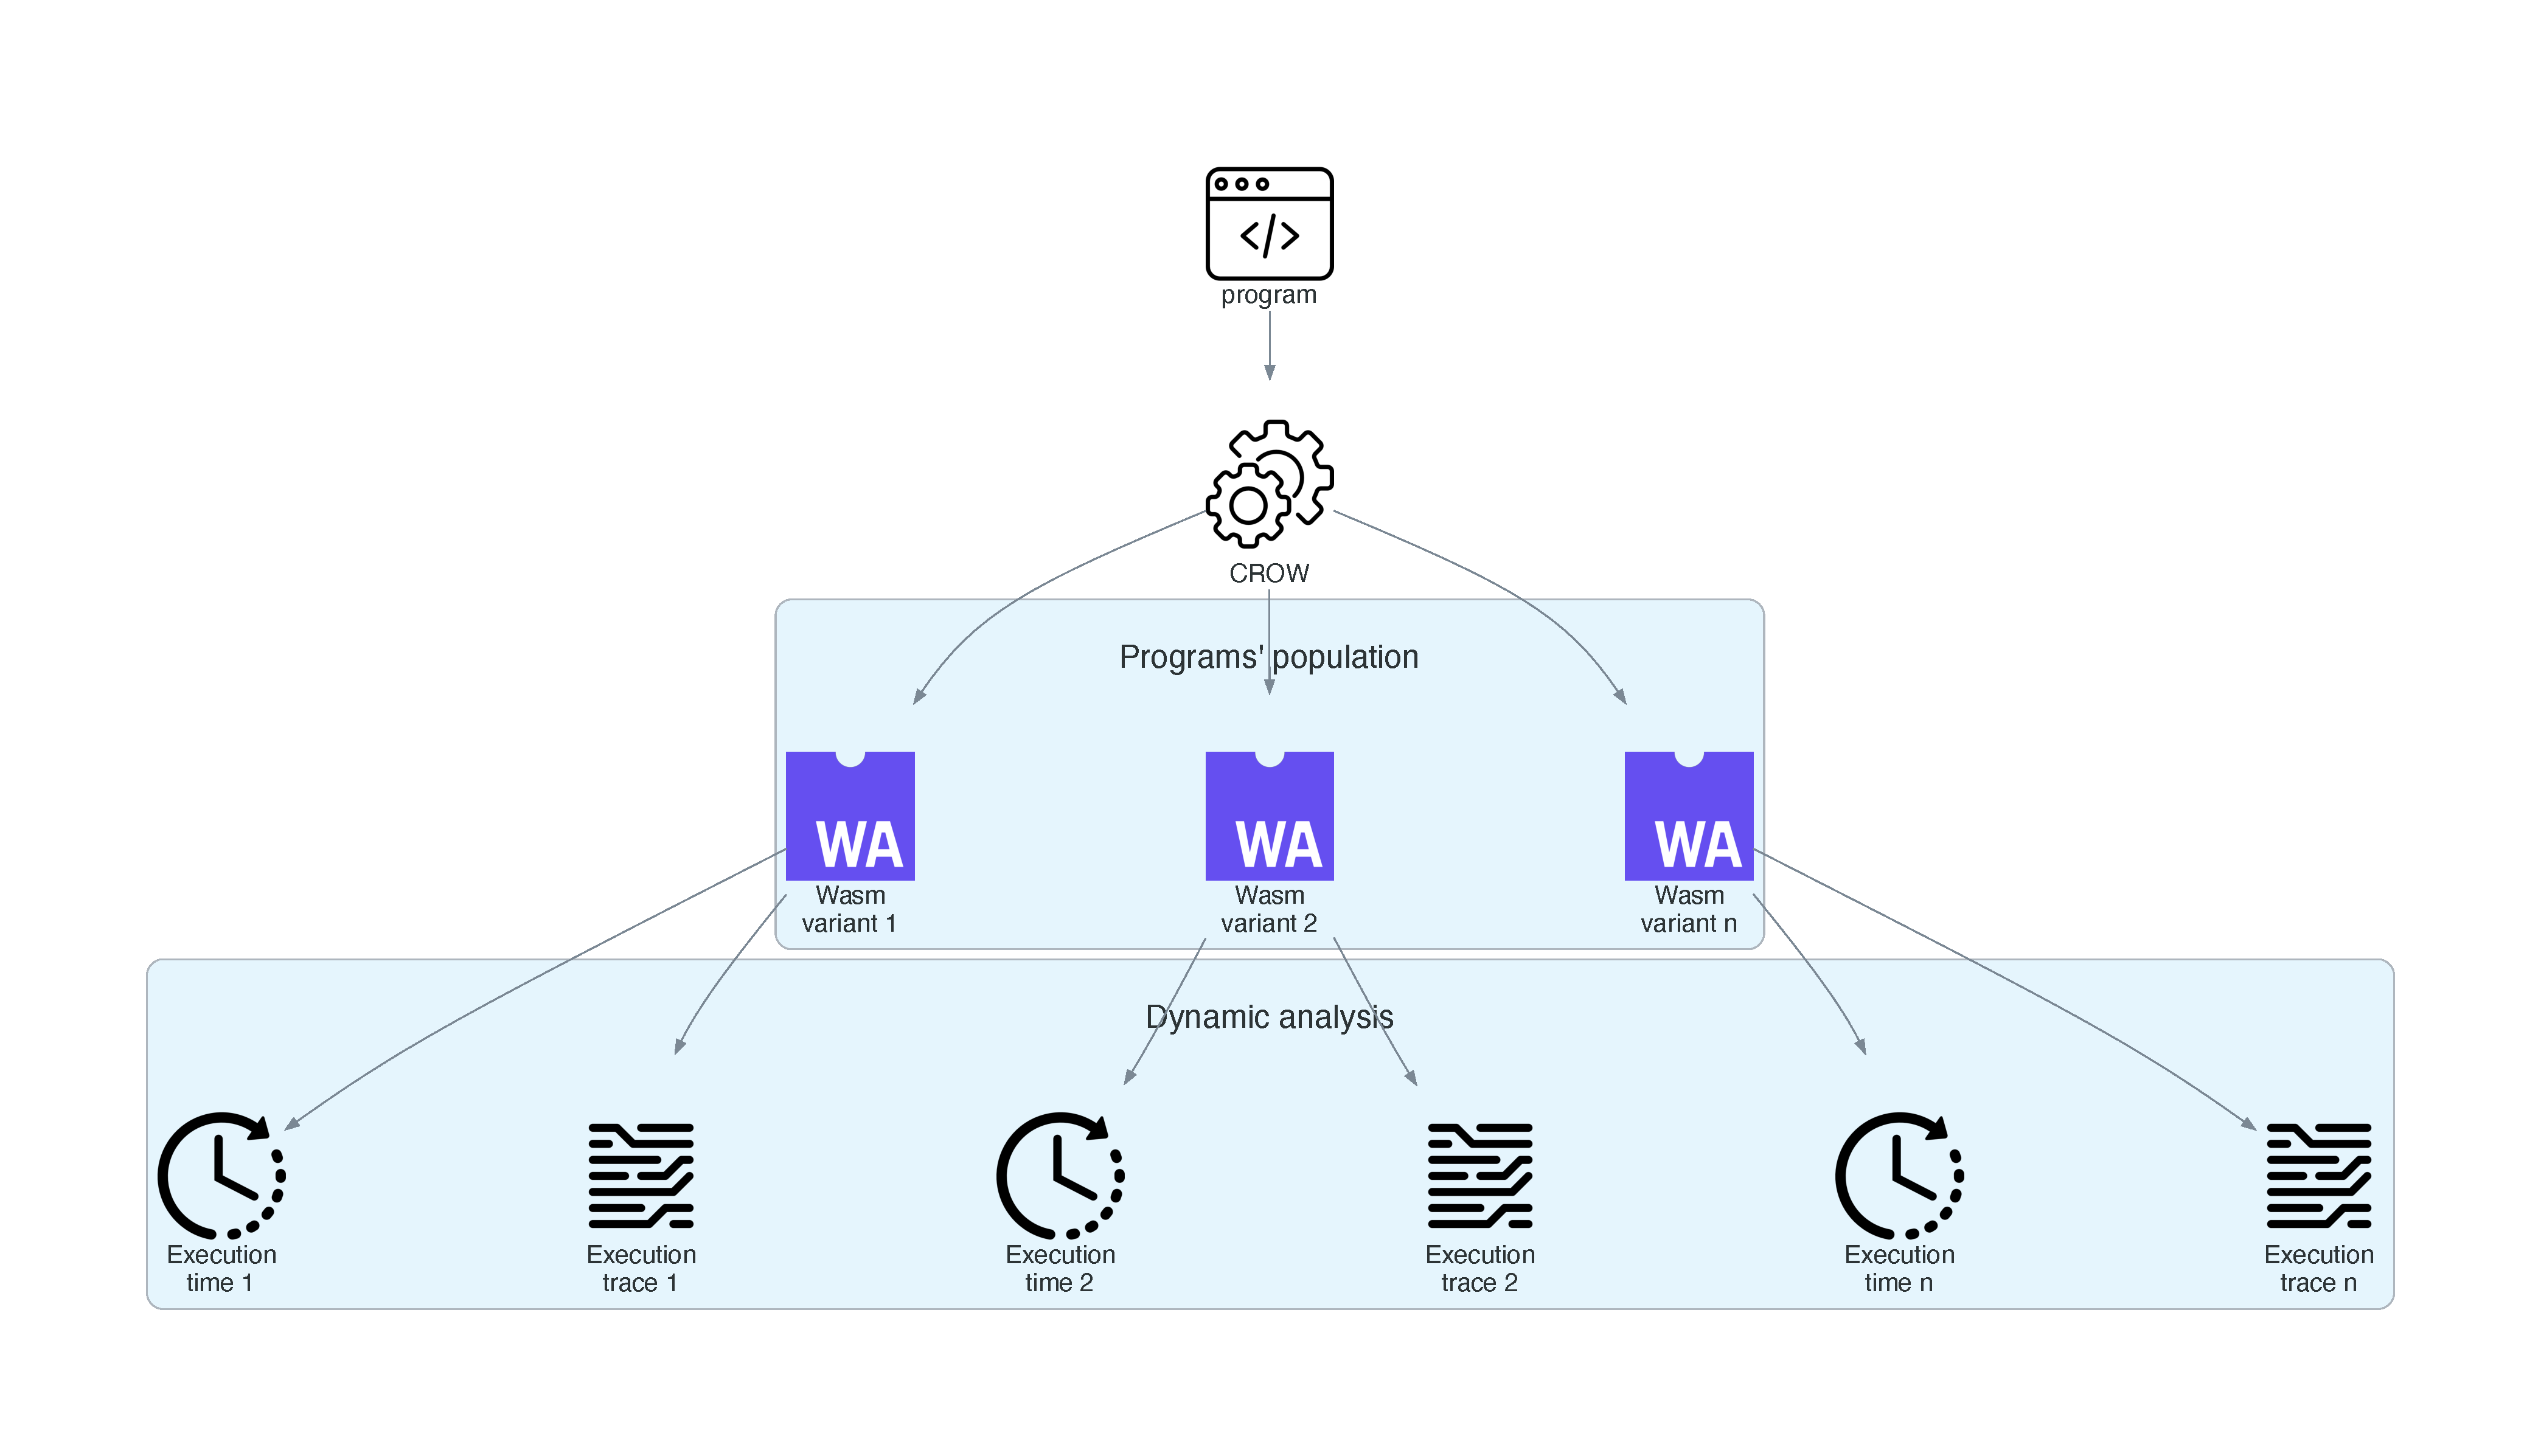
\includegraphics[width=\linewidth]{diagrams/Rq2.pdf}
    \caption{Dynamic analysis for RQ2.}
    \label{diagrams:protocol:rq2}
\end{figure*}

In this second research question, we investigate to what extent the artificially created variants are dynamically different between them and the original program. To conduct this research question, we could separate our experiments into two fields as \autoref{diagrams:protocol:rq2} illustrates: static analysis and dynamic analysis. 
The static analysis focuses on the appreciated differences among the program variants, as well as between the variants and the original program, and we address it in answering RQ1. 
With RQ2, we focus on the last category, the dynamic analysis of the generated variants. This decision is supported because dynamic analysis complements RQ1 and, it is essential to provide a full understanding of diversification.
We use the original functions from \corpusrosetta corpus described in \autoref{section:crow:corpora} and their variants generated to answer RQ1. 
We use only \corpusrosetta to answer RQ2 because this corpus is composed of simple programs that can be executed directly without user interaction, \ie we only need to call the interpreter passing the \wasm binary to it. 

\todo{Motivate, Increasing attack surface does not necesarilly has an impact on defence. For example, reordering instructions for code blocks that are never executed does not impact attacker}

To dynamically compare programs and their variants, we execute each program on each programs' population to collect and execution times. We define execution trace and execution time in the following section.
%\todo{vague and subjective, avoid or elaborate: We perform fine-grained} comparisons by comparing the traces and execution times for all pairs of programs. Therefore, the defined metrics are formulated to support a pairwise comparison strategy.
%In the following, we define the metrics used to answer RQ2.

\subsection*{Metrics}
\label{rq2:metrics}

We compare the execution traces of two any programs of the same population with a global alignment metric. We propose a global alignment approach using Dynamic Time Warping (DTW).
Dynamic Time Warping \cite{NEEDLEMAN1970443} computes the global alignment between two sequences. It returns a value capturing the cost of this alignment, which is a distance metric. The larger the DTW distance, the more different the two sequences are.
DTW has been used for comparing traces in different domains. For software, De A. Maia \etal \cite{ Maia08usinga} proposed to identify similarity between programs from execution traces.
In our experiments, we define the traces as the sequence of the stack operations during runtime, \ie the consecutive list of \texttt{push} and \texttt{pop} operations performed by the \wasm engine during the execution of the program.
In the following, we define the $\DTW$ metric. 
 


\todo{before, define this and give an illutrative listing plus, says how you collect those traces, that's part of the protocol: between the stack operation traces }

\begin{metric}{\DTW{}:}
\label{metric:stack}
\normalfont 
	Given two programs P and P' from the same program's population, \DTW{}(P,P'), computes the DTW distance collected during their execution. \\
	A \DTW{} of $0$ means that both traces are identical.
	The higher the value, the more different the traces. 
\end{metric}



Moreover, we use the execution time distribution of the programs in the population to complement the answer to RQ2. For each program pair in the programs' population, we compare their execution time distributions. We define the execution time as follows:

\begin{metric}{Execution time:}\label{metric:time}
    \normalfont 
	Given a \wasm program P, the execution time is the time spent to execute the binary.
\end{metric}



%\subsection{Variants preservation}

\subsection*{Protocol}

% Dynamic
To compare program and variants behavior during runtime, we analyze all the unique program variants generated to answer RQ1 in a pairwise comparison using the value of aligning their execution traces (\autoref{metric:stack}). We use SWAM\footnote{\url{https://github.com/satabin/swam}} to execute each program and variant to collect the stack operation traces. SWAM is a \wasm interpreter that provides functionalities to capture the dynamic information of \wasm program executions, including the virtual stack operations.
% \todo{Can the reader runderstand that? We want to remark that we only collect the stack operation traces due to the memory-agnosticism of our approach to generate variants. Our approach does not change the memory-like operations of the original code.}

Furthermore, we collect the execution time, \autoref{metric:time}, for all programs and their variants. We compare the collected execution time distributions between programs using a Mann-Withney U test \cite{mann1947} in a pairwise strategy.

%\todo{Maybe the first time that Mann-Withney is mentioned I should describe what it is}

 


\section{\rqthree}
\label{rq3:method}


\todo{The last method is too short}


\newcommand{\mewe}{MEWE\xspace}

\begin{figure}[h]
    \centering
    \includegraphics[width=0.8\linewidth]{diagrams/Rq3.pdf}
    \caption{Multivariant binary creation and workflow for RQ3 answering.}
    \label{diagrams:protocol:rq3}
\end{figure}

In the last research question, we study whether the created variants can be used in real-world applications and what properties offer the composition of the variants as multivariant binaries. \todo{Not defined: We build multivariant binaries}, and we deploy and execute them at the Edge. The process of \emph{mixing} multiple variants into one multivariant binary is an essential contribution of the thesis that is presented in details in \cite{2021arXiv210808125C}. RQ3 focuses on analyzing the impact of this contribution on execution times. To answer RQ3, we use the variants generated for the programs of \corpussodium and \corpusqrcode corpora, we take $2 + 5$ programs interconnecting the LLVM bitcode modules (mentioned in \autoref{table:corpora}). We illustrate the protocol to answer RQ3 in \autoref{diagrams:protocol:rq3} starting from the creation of the programs' population.



%The workflow starts by using the programs' population of each program generated in RQ1 to create the multivariant binaries. We deploy the multivariant binaries at the Edge, and we collect their execution times. We measure the differences for the execution times on the edge. Then, we discuss how multivariant binaries contribute to less predictable timing side-channels.

\subsection*{Metrics}

We use the execution time of the multivariant binaries to answer RQ3. We use the same metric defined in \autoref{metric:time} for the execution time of multivariant binaries.

\subsection*{Protocol}


We run the experiments to answer RQ3 on the Edge, \todo{too fast. tell the reader why you need HTTP now: executing the multivariant binaries as end-to-end HTTP services.} 
The execution times are measured at the backend space, \ie we collect the execution times inside the Edge node and not from the client computer. Therefore, we instrument the binaries to return the execution time as an HTTP header. We do this process for the original program and its multivariant binary. We deploy and execute the original and the multivariant binaries on 64 edge nodes located around the world \todo{Add illustrative map}.


We collect 100k execution times for each binary \todo{Why? Cite blackhat paper and the need of 1 million traces multiplied by the number of nodes}, both the original and multivariant binaries.
We perform a Mann-Withney U test \cite{mann1947} to compare both execution time distributions. 
If the P-value is lower than 0.05, the two compared distributions are different.

%\pagebreak

\section*{Conclusions}

This chapter presents the methodology we follow to answer our three research questions. We first describe and propose the corpora of programs used in this work. We propose to measure the ability of our approach to generate variants out of \py{303  + \libsodiumfunctions + \qrcodefunctions} functions of our corpora. Then, we suggest using the generated variants to study to what extent they offer different observable behavior through dynamic analysis. We propose a protocol to study the impact of the composition variants in a multivariant binary deployed at the Edge. Besides, we enumerate and enunciate the properties and metrics that might lead us to answer the impact of automatic diversification for \wasm programs. In the next chapter, we present and discuss the results obtained with this methodology.


%\todo{Add the unique and the total.}
%\todo{Change metrics and the name of dt\_dyn.}
%\todo{Remove growing factor.}
%\todo{Explain what a quantile-quantile plot is.}

\clearpage
%\chapter{Methodology} 
\label{chapter:method}

\pagestyle{plain}
% Define some numbers here for the autmation of the tables
\newcommand{\libsodiumfunctions}{869}
\newcommand{\qrcodefunctions}{1849}
\newcommand{\allmewefunctions}{\libsodiumfunctions + \qrcodefunctions}

% Execute a python script for small calculations
\newcommand{\py}[1]{\input{|python3 interpreter.py #1}}
\newcommand{\fromjson}[2]{\input{| jq -r '#2' '#1}}

\newcommand{\corpusrosetta}{Rosetta\xspace}
\newcommand{\corpussodium}{Libsodium\xspace}
\newcommand{\corpusqrcode}{QrCode\xspace}


\newcommand{\DTWStatic}{dt\_static\xspace}
\newcommand{\DTW}{TraceDiff\xspace}
\renewcommand{\tool}{CROW\xspace}

%\todo{Recheck the selection of the modules for sodium}

%This chapter investigates whether we can artificially create program variants through semantically equivalent code transformations. We propose a framework to generate program variants functionally equivalent to their original.
%We introduce the retargeting of a superoptimizer, using its exhaustive search strategy to provide semantically equivalent code transformations. 
%The presented methodology and transformation tool, CROW, are contributions to this thesis.
%We evaluate the usage of CROW on two corpora of open-source and nature diverse programs. 
In this chapter, we present our methodology to answer the research questions enunciated in \autoref{intro:definition:rq}.
We investigate three research questions. In the first question, we aim to investigate the static differences between variants. We evaluate the code properties the lead less or more software diversification.
Our second research question focuses on comparing their behavior during their execution, complementing our first research question. The generated variants should be statically different, but also should provide different observable behavior. 
The final research question evaluates the feasibility of using the program variants in security-sensitive environments. We evaluate our generated program variants in an Edge-Cloud computing platform proposing a novel multivariant execution approach.

% \todo{too generic: READ AGAIN to see how to land this
The main objective of this thesis is to study the feasibility of automatically creating program variants out of preexisting program sources. To achieve this objective,
we use the empirical method \cite{Runeson2020}, proposing a solution and evaluating it through quantitative analyzes in case studies. We follow an iterative and incremental approach on the selection of programs for our corpora. To build our corpora, we find a representative and diverse set of programs to generalize, even when it is unrealistic following an empirical approach, as much as possible our results.
We first enunciate the corpora we share along this work to answer our research questions. Then, we establish the metrics for each research question, set the configuration for the experiments, and describe the protocol.

% Our approach lies under \textit{Design Science} \cite{Runeson2020}, in terms of empirical validation, the scope of the design knowledge gained in a study can be extended by systematically extending the scope of the valudation in subsequent studies. Thus, the size of our corpora can be extended to increase the knowledge of the research area.


\section{Corpora}
\label{section:crow:corpora}

Our experiments assess the impact of artificially created diversity. The first step is to build a suitable corpus of programs' seeds to generate the variants. Then, we answer all our research questions with three corpora which follow two main properties: 1) \emph{functionally diverse:} the selection of the programs is not biased by functionally fixed tasks, for example, the programs in one of our corpora solve from the \textit{Babbage} problem to \textit{Convex Hull} calculation; and 2) \emph{representative:} our corpora have 3021 programs that can be ported to \wasm, representing approximately 40\% of the unique Wasm binaries in the wild \cite{Hilbig2021AnES}.


We build our three corpora in an escalating strategy based on the merging of our previous publications. The first corpus is diverse and contains simple programs in terms of code size, making them easy to manually analyze. The second corpus is a project meant for security-sensitive applications. The third corpus is a QR encoding decoding algorithm. 
%The work of Hilbig \etal \cite{Hilbig2021AnES} shows that approximately 65\% of all \wasm programs come out of C/C++ source code through the LLVM pipeline, and more than 75\% if the Rust language is included. Therefore, all modules in the corpora are considered to come along the LLVM pipeline. 
In the following, we describe the filtering and description of each corpus.

\begin{enumerate}
    \item \textbf{\corpusrosetta}: We take programs from the Rosetta Code project\footnote{\url{http://www.rosettacode.org/wiki/Rosetta_Code}}. This website hosts a curated set of solutions for specific programming tasks in various programming languages. It contains many tasks, from simple ones, such as adding two numbers, to complex algorithms like a compiler lexer. We first collect all C programs from the Rosetta Code, representing $989$ programs as of 01/26/2020. We then apply several filters: the programs should successfully compile and, they should not require user inputs to automatically execute them, the programs should terminate and should not result in non-deterministic results. 
    
    The result of the filtering is a corpus of 303 C programs. All programs include a single function in terms of source code. These programs range from $7$ to $150$ lines of code.

    \item \textbf{\corpussodium}: This project is encryption, decryption, signature, and password hashing library implemented in 102 separated modules. The modules have between $8$ and $2703$ lines of code per function. This project is selected based on two main criteria: first, its importance for security-related applications, and second, its suitability to collect the modules in LLVM intermediate representation. %We select 5 programs that interconnect the 102 modules of the project.

    \item \textbf{\corpusqrcode}: This project is a QrCode and MicroQrCode generator written in Rust. This project contains 2 modules having between $4$ and $725$ lines of code per function. As \corpussodium, we select this project due to its suitability for collecting the modules in their LLVM representation. Remarkably, this project increases the complexity of the previously selected projects due to its integration with the generation of images.
    
\end{enumerate}

In \autoref{table:corpora} we listed the corpus name, the language of the programs in the corpus, the number of modules, the total number of functions, the range of lines of code, and the original location of the corpus. 


%The first corpus, \textbf{CROW prime}, . The second corpus, \textbf{MEWE prime}, is part of the MEWE contribution \cite{}. In \autoref{table:corpora} we summarize the selection criteria, and we mention each corpus properties. With both corpora we evaluate CROW with a total of $303 + \py{\allmewefunctions}$ functions. 

\begin{table}[h]
    \renewcommand{\arraystretch}{1.0}
    \small
    \centering
    \begin{tabular}{l | p{1cm} | l | l | l | p{3.2cm}}
        Corpus & Lang. & No. modules & No. functions & LOC range & Location \\
        \midrule
            % CROW
            \corpusrosetta & C &
            - %\footnote{ The concept of module does not apply for this corpus programs. } 
            &
            303  & 
            7 - 
            150 & 
            \url{https://github.com/KTH/slumps/tree/master/benchmark_programs/rossetta/valid/no_input}\\
        \hline
        \corpussodium & LLVM IR + Rust &
        102 &
        869  &
        8 - 2703 &   
        \url{https://github.com/jedisct1/libsodium/tree/2b5f8f2b6810121c2d9a8cc8a392e01f4d3de433 }\\
        \hline
        \corpusqrcode & LLVM IR + Rust &
        2 &
        1849  & 
        4 - 725   & 
        \url{https://github.com/kennytm/qrcode-rust/commit/faa4397ba7c5f441cb9a2b436c1e84a0d52ae942} \\
        % Total stats
        \hline
        \hline
        \textbf{Total} & & 
        & 
        \py{ 303 + \qrcodefunctions + \libsodiumfunctions} &  
        &     \\

    \end{tabular}
    \caption{Corpora description. The table is composed by the name of the corpus, programming language of the programs in the corpus, the number of modules, the number of functions, the lines of code range and the location of the corpus.}
    \label{table:corpora}
\end{table}


\section{\rqone}
\label{rq1:method}

\begin{figure}[h]
    \centering
    \includegraphics[height=4.1in]{diagrams/RQ1.pdf}
    \caption{The program variants generation for RQ1.}
    \label{diagrams:protocol:rq1}
\end{figure}


This research question investigates whether we can artificially generate program variants for \wasm. We use CROW to generate variants from an original program, written in C/C++ in the case of the \corpusrosetta corpus and LLVM bitcode modules in the case of the \corpussodium and \corpusqrcode. 
In \autoref{diagrams:protocol:rq1} we illustrate the workflow to generate \wasm\ program variants. We pass each function of the corpora to CROW as a program to diversify. To answer RQ1, we study the outcome of this pipeline, the generated \wasm\ variants. 


\subsection*{Metrics}

To assess our approach's ability to generate \wasm\ binaries that are statically different, we compute the number of variants and the number of unique variants for each original function of each corpus. 
On top, we define the aggregation of these former two values to quantitatively evaluate RQ1 at the corpus level. 

We start by defining what a program's population is. This definition can be applied in general to any collection of variants of the same program. All definitions are based upon bytecodes and not the source code of the programs.

\begin{definition}{Program's population $M(P)$:}\label{def:rq1:programspopulation}
    \normalfont 
    Given a program P and its generated variants $v_i$, the program's population is defined as:\\
    $$
        M(P)=\{v_i\ \text{where $v_i$ is a variant of P}\}
    $$

    Notice that the program's population includes the original program P.
\end{definition}

Beyond the program's population, we also want to compare how many program variants are unique. The subset of unique programs in the program's population hints how the variants are different between them and not only against the original program. For example, imagine a program $P$ with two program variants $V_1$ and $V_2$, the program population is composed by $\{P, V_1 \text{ and } V_2\}$, where $V_1$ is different from $P$, and $V_2$ is different from $P$. $V_1$ is either equal or different from $V_2$, the program's population still be the same. If $V_1$ and $V_2$ are equal, then only one unique variant is generated,

%\todo{
%   clarify source code versus byte code for earch definition.

%why are those definitions important? interesting? why do you introduce them?
%}
%Notice that all metrics over programs and their variants make sense only at the population level. Therefore, we compare semantically equivalent programs from the same population.

%\todo{
%   difference unclear or trivial.

%do you need source code versus bytecode?

%clarify
%}

\begin{definition}{Program's unique population $U(P)$:}\label{def:rq1:programsuniquepopulation}
    \normalfont 
    Given a program P and its program's population $M(P)$, the program's unique population is defined as.\\
    $$
        U(P)=\{v\ \in\ M(P)\}
    $$
    such that $\forall v_i,v_j \in U(P)$, $v_i \neg v_j$ $\Rightarrow$ $md5sum(v_i) \ne md5sum(v_j)$.
    $Md5sum(v)$ is the md5 hash calculated over the bytecode stream of the program file $v$. Notice that the original program $P$ is included in $U(P)$.

\end{definition}

\begin{metric}{Program's population size $S(P)$:}\label{metric:rq1:PS}
    \normalfont 
    Given a program P and its program's population $M(P)$ according to \autoref{def:rq1:programspopulation}, the program's population size is defined as.\\
    $$
        S(P)=|M(P)|
    $$
\end{metric}


\begin{metric}{Program's unique population size $US(P)$:}\label{metric:rq1:UP}
    \normalfont 
    Given a program P and its program's unique population $U(P)$ according to \autoref{def:rq1:programsuniquepopulation}, the program's unique population size is defined as.\\
    $$
        US(P)=|U(P)|
    $$
\end{metric}

\newcommand{\corpuspopulationsizename}{Corpus population size\xspace}
\newcommand{\corpusuniquepopulationsizename}{Corpus unique population size\xspace}

\begin{metric}{\corpuspopulationsizename$CS(C)$:}\label{metric:rq1:corpus_pop}
    \normalfont 
    Given a program's corpus $C$, the corpus population size is defined as the sum of all program's population sizes over the corpus $C$:\\
    $$
        CS(C)=\Sigma{S(P)}\ \forall\ P\ \in\ C
    $$
\end{metric}

\begin{metric}{\corpusuniquepopulationsizename$UCS(C)$:}\label{metric:rq1:corpus_pop_unique}
    \normalfont 
    Given a program's corpus $C$, the corpus unique population size is defined as the sum of all program's unique population sizes over the corpus $C$ :\\
    $$
    UCS(C)=\Sigma{US(P)}\ \forall\ P\ \in\ C
    $$
\end{metric}


\subsection*{Protocol}
To generate program variants, we synthesize programs with an enumerative strategy, checking each synthesis for equivalence modulo input \cite{Li2018} against the original program, as it is described in \autoref{section:crow}. For obvious reasons, this space is nearly impossible to explore in a reasonable time as soon as the limit of instructions increases.
Therefore, we use two parameters to control the size of the search space and hence the time required to traverse it.
On the one hand, one can limit the size of the variants. On the other hand, one can limit the set of instructions used for the synthesis. In our experiments for RQ1, we use all instructions in the CROW diversifier synthesis.


The former parameter allows us to find a trade-off between the number of variants that are synthesized and the time taken to produce them. For the current evaluation, given the size of the corpus and the properties of its programs, we set the exploration time to 1 hour maximum per function for \corpusrosetta. In the cases of \corpussodium\ and\ \corpusqrcode, we set the timeout to 5 minutes per function. The decision behind the usage of lower timeout for \corpussodium
and \corpusqrcode is motivated by the properties listed in \autoref{table:corpora}. The latter two corpora are remarkably larger regarding the number of instructions and functions. 

We pass each of the $303 + \libsodiumfunctions + \qrcodefunctions$ functions in the corpora to CROW, as \autoref{diagrams:protocol:rq1} illustrates, to synthesize program variants. We calculate the \emph{Corpus population size} (\autoref{metric:rq1:corpus_pop}) and \emph{Corpus unique population size} (\autoref{metric:rq1:corpus_pop_unique}) for each corpus and conclude by answering RQ1.



\section{\rqtwo}
\label{rq2:method}


\begin{figure*}[h]
    \centering
    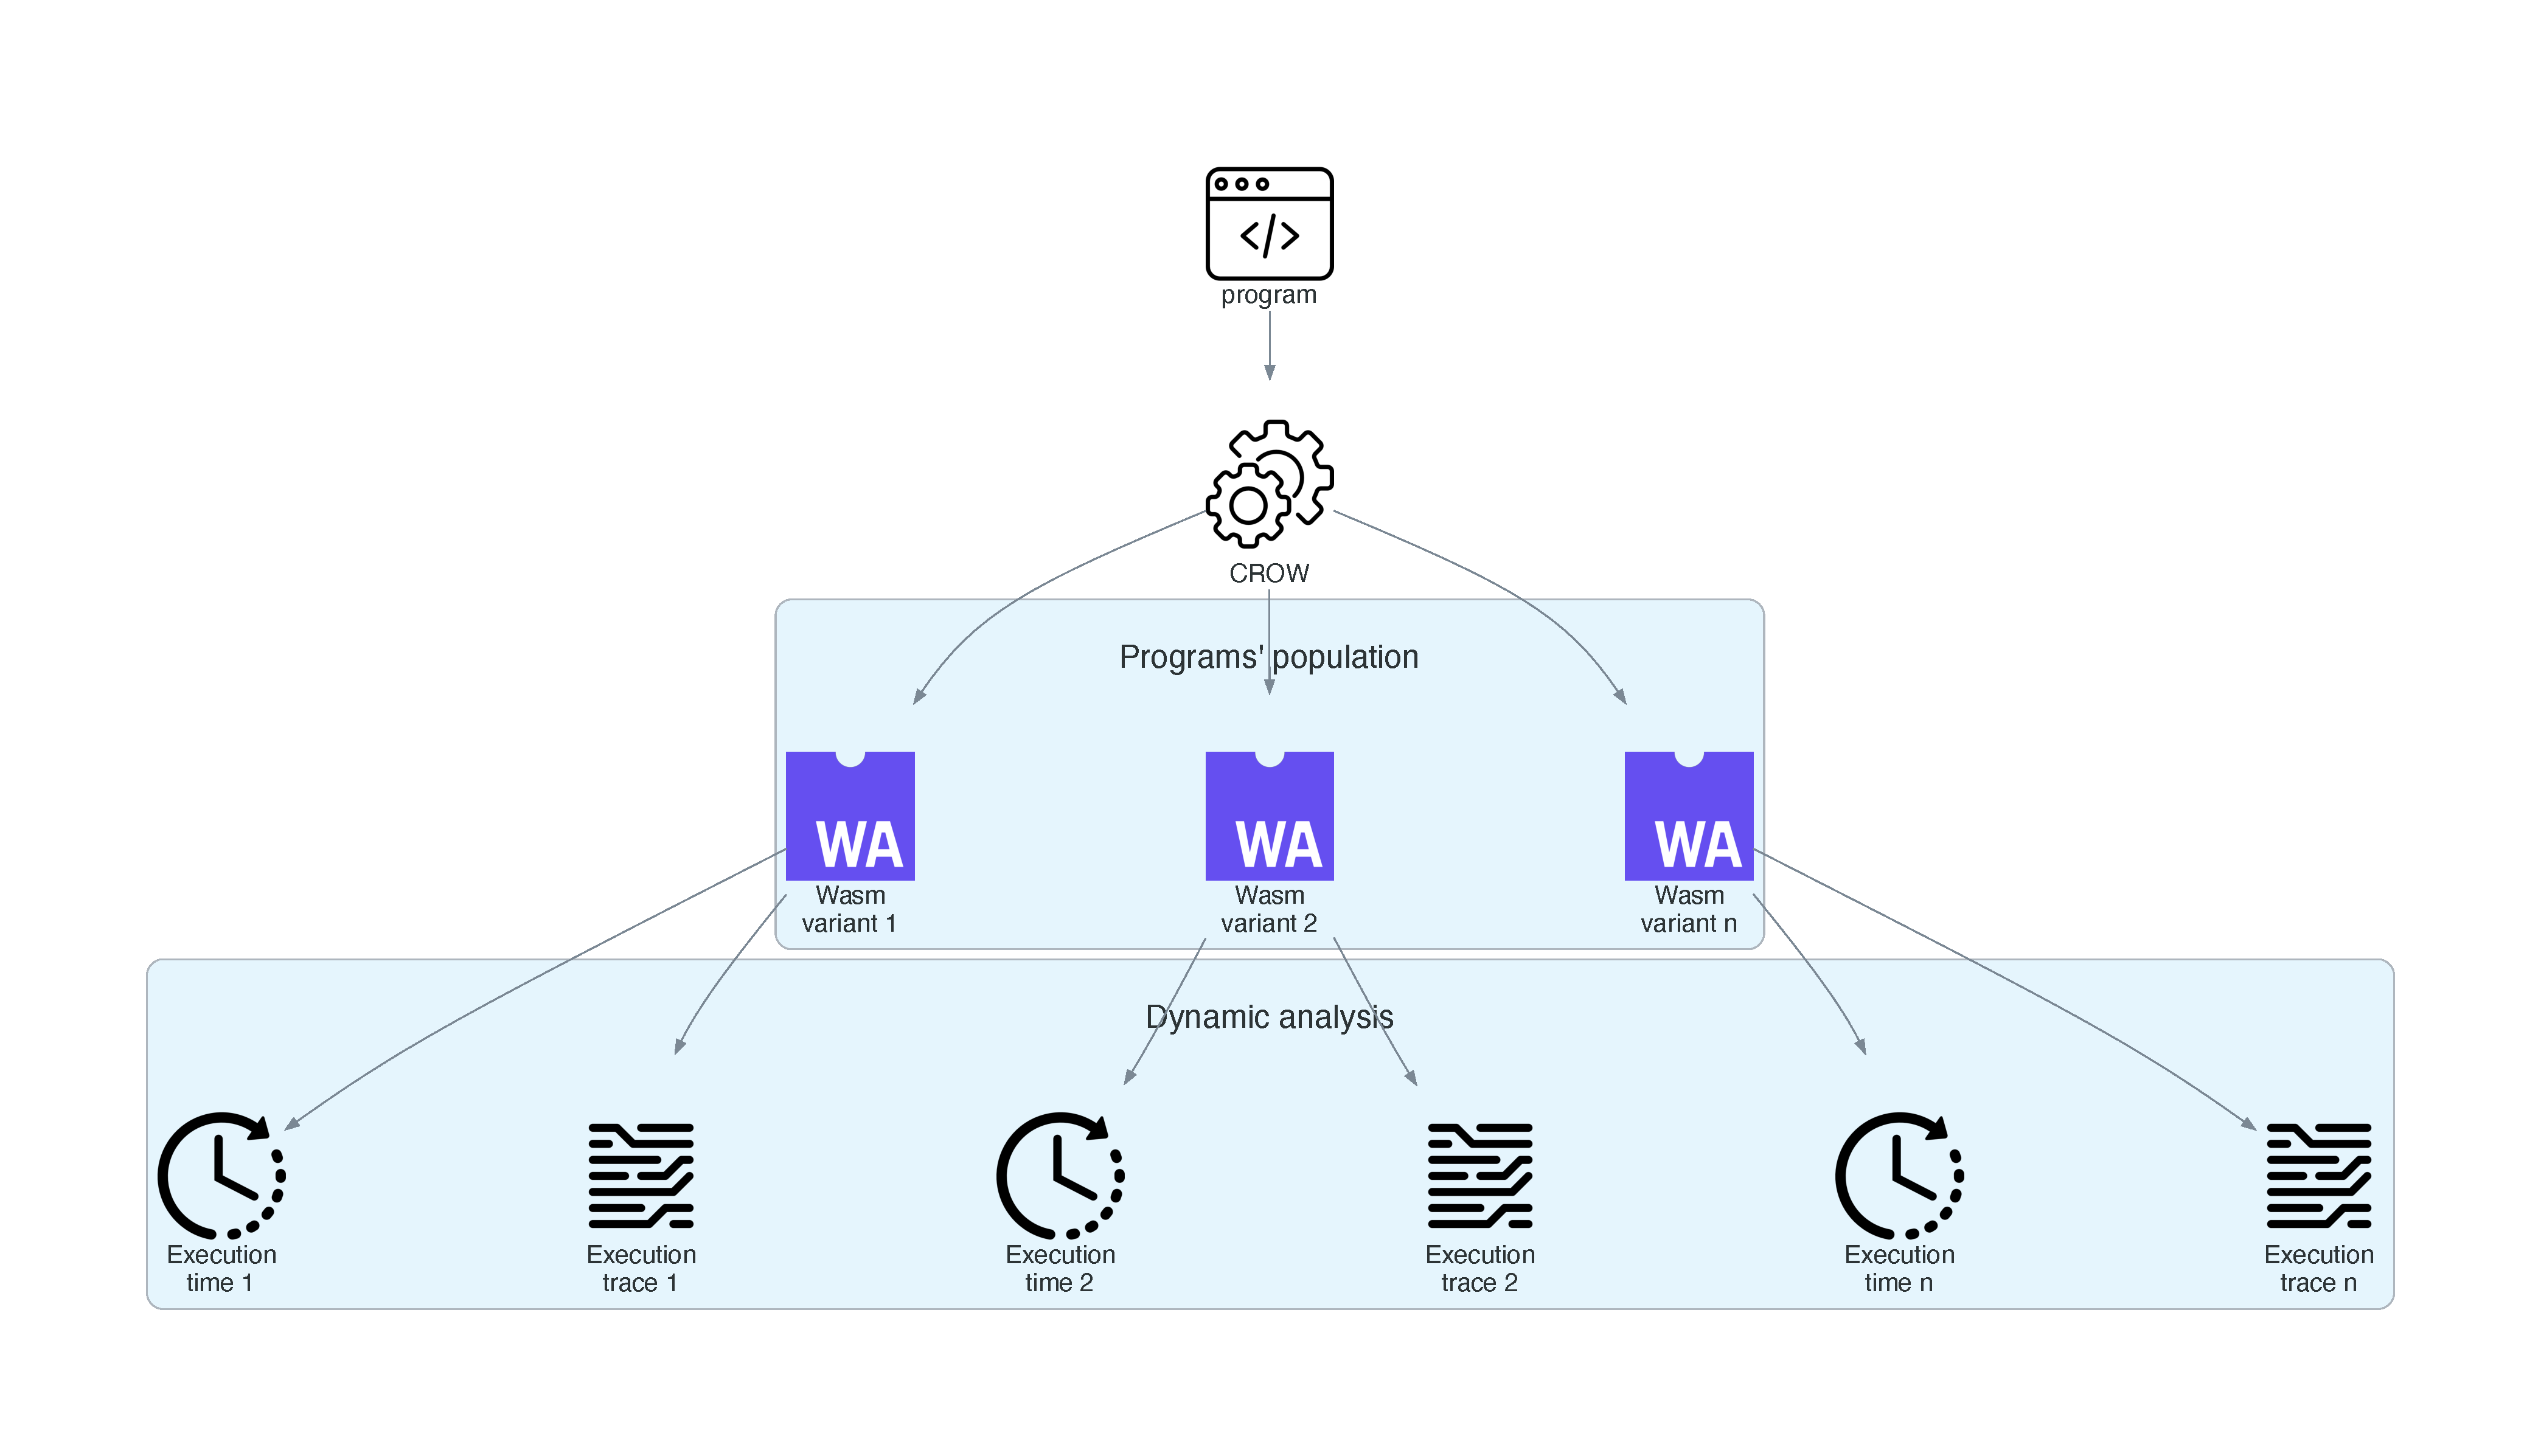
\includegraphics[width=\linewidth]{diagrams/Rq2.pdf}
    \caption{Dynamic analysis for RQ2.}
    \label{diagrams:protocol:rq2}
\end{figure*}

In this second research question, we investigate to what extent the artificially created variants are dynamically different between them and the original program. To conduct this research question, we could separate our experiments into two fields as \autoref{diagrams:protocol:rq2} illustrates: static analysis and dynamic analysis. 
The static analysis focuses on the appreciated differences among the program variants, as well as between the variants and the original program, and we address it in answering RQ1. 
With RQ2, we focus on the last category, the dynamic analysis of the generated variants. This decision is supported because dynamic analysis complements RQ1 and, it is essential to provide a full understanding of diversification.
We use the original functions from \corpusrosetta corpus described in \autoref{section:crow:corpora} and their variants generated to answer RQ1. 
We use only \corpusrosetta to answer RQ2 because this corpus is composed of simple programs that can be executed directly without user interaction, \ie we only need to call the interpreter passing the \wasm binary to it. 

\todo{Motivate, Increasing attack surface does not necesarilly has an impact on defence. For example, reordering instructions for code blocks that are never executed does not impact attacker}

To dynamically compare programs and their variants, we execute each program on each programs' population to collect and execution times. We define execution trace and execution time in the following section.
%\todo{vague and subjective, avoid or elaborate: We perform fine-grained} comparisons by comparing the traces and execution times for all pairs of programs. Therefore, the defined metrics are formulated to support a pairwise comparison strategy.
%In the following, we define the metrics used to answer RQ2.

\subsection*{Metrics}
\label{rq2:metrics}

We compare the execution traces of two any programs of the same population with a global alignment metric. We propose a global alignment approach using Dynamic Time Warping (DTW).
Dynamic Time Warping \cite{NEEDLEMAN1970443} computes the global alignment between two sequences. It returns a value capturing the cost of this alignment, which is a distance metric. The larger the DTW distance, the more different the two sequences are.
DTW has been used for comparing traces in different domains. For software, De A. Maia \etal \cite{ Maia08usinga} proposed to identify similarity between programs from execution traces.
In our experiments, we define the traces as the sequence of the stack operations during runtime, \ie the consecutive list of \texttt{push} and \texttt{pop} operations performed by the \wasm engine during the execution of the program.
In the following, we define the $\DTW$ metric. 
 


\todo{before, define this and give an illutrative listing plus, says how you collect those traces, that's part of the protocol: between the stack operation traces }

\begin{metric}{\DTW{}:}
\label{metric:stack}
\normalfont 
	Given two programs P and P' from the same program's population, \DTW{}(P,P'), computes the DTW distance collected during their execution. \\
	A \DTW{} of $0$ means that both traces are identical.
	The higher the value, the more different the traces. 
\end{metric}



Moreover, we use the execution time distribution of the programs in the population to complement the answer to RQ2. For each program pair in the programs' population, we compare their execution time distributions. We define the execution time as follows:

\begin{metric}{Execution time:}\label{metric:time}
    \normalfont 
	Given a \wasm program P, the execution time is the time spent to execute the binary.
\end{metric}



%\subsection{Variants preservation}

\subsection*{Protocol}

% Dynamic
To compare program and variants behavior during runtime, we analyze all the unique program variants generated to answer RQ1 in a pairwise comparison using the value of aligning their execution traces (\autoref{metric:stack}). We use SWAM\footnote{\url{https://github.com/satabin/swam}} to execute each program and variant to collect the stack operation traces. SWAM is a \wasm interpreter that provides functionalities to capture the dynamic information of \wasm program executions, including the virtual stack operations.
% \todo{Can the reader runderstand that? We want to remark that we only collect the stack operation traces due to the memory-agnosticism of our approach to generate variants. Our approach does not change the memory-like operations of the original code.}

Furthermore, we collect the execution time, \autoref{metric:time}, for all programs and their variants. We compare the collected execution time distributions between programs using a Mann-Withney U test \cite{mann1947} in a pairwise strategy.

%\todo{Maybe the first time that Mann-Withney is mentioned I should describe what it is}

 


\section{\rqthree}
\label{rq3:method}


\todo{The last method is too short}


\newcommand{\mewe}{MEWE\xspace}

\begin{figure}[h]
    \centering
    \includegraphics[width=0.8\linewidth]{diagrams/Rq3.pdf}
    \caption{Multivariant binary creation and workflow for RQ3 answering.}
    \label{diagrams:protocol:rq3}
\end{figure}

In the last research question, we study whether the created variants can be used in real-world applications and what properties offer the composition of the variants as multivariant binaries. \todo{Not defined: We build multivariant binaries}, and we deploy and execute them at the Edge. The process of \emph{mixing} multiple variants into one multivariant binary is an essential contribution of the thesis that is presented in details in \cite{2021arXiv210808125C}. RQ3 focuses on analyzing the impact of this contribution on execution times. To answer RQ3, we use the variants generated for the programs of \corpussodium and \corpusqrcode corpora, we take $2 + 5$ programs interconnecting the LLVM bitcode modules (mentioned in \autoref{table:corpora}). We illustrate the protocol to answer RQ3 in \autoref{diagrams:protocol:rq3} starting from the creation of the programs' population.



%The workflow starts by using the programs' population of each program generated in RQ1 to create the multivariant binaries. We deploy the multivariant binaries at the Edge, and we collect their execution times. We measure the differences for the execution times on the edge. Then, we discuss how multivariant binaries contribute to less predictable timing side-channels.

\subsection*{Metrics}

We use the execution time of the multivariant binaries to answer RQ3. We use the same metric defined in \autoref{metric:time} for the execution time of multivariant binaries.

\subsection*{Protocol}


We run the experiments to answer RQ3 on the Edge, \todo{too fast. tell the reader why you need HTTP now: executing the multivariant binaries as end-to-end HTTP services.} 
The execution times are measured at the backend space, \ie we collect the execution times inside the Edge node and not from the client computer. Therefore, we instrument the binaries to return the execution time as an HTTP header. We do this process for the original program and its multivariant binary. We deploy and execute the original and the multivariant binaries on 64 edge nodes located around the world \todo{Add illustrative map}.


We collect 100k execution times for each binary \todo{Why? Cite blackhat paper and the need of 1 million traces multiplied by the number of nodes}, both the original and multivariant binaries.
We perform a Mann-Withney U test \cite{mann1947} to compare both execution time distributions. 
If the P-value is lower than 0.05, the two compared distributions are different.

%\pagebreak

\section*{Conclusions}

This chapter presents the methodology we follow to answer our three research questions. We first describe and propose the corpora of programs used in this work. We propose to measure the ability of our approach to generate variants out of \py{303  + \libsodiumfunctions + \qrcodefunctions} functions of our corpora. Then, we suggest using the generated variants to study to what extent they offer different observable behavior through dynamic analysis. We propose a protocol to study the impact of the composition variants in a multivariant binary deployed at the Edge. Besides, we enumerate and enunciate the properties and metrics that might lead us to answer the impact of automatic diversification for \wasm programs. In the next chapter, we present and discuss the results obtained with this methodology.


%\todo{Add the unique and the total.}
%\todo{Change metrics and the name of dt\_dyn.}
%\todo{Remove growing factor.}
%\todo{Explain what a quantile-quantile plot is.}

\clearpage
%\chapter{Conclusions}

%\Chapter{Variant's application}{RQ3. To what extent the generated variants can be used in security vulnerable applications?} 

%\section{Security MTD}

%\section{Reliability (CVE + fuzz) future work}

%\bibliographystyle{IEEEtranS} % this is just an example, other styles can be used as well
\bibliographystyle{apalike} % this is just an example, other styles can be used as well
\bibliography{Lic} % calls the separate document named Lic.bbl

%\backmatter % should be used for the actual thesis, separate documents can be added without the numbering, similar to the \frontmatter
%\appendix{\chapter{Appended Papers}

Write your conclusion here...}
% \appendix


%\addcontentsline{toc}{chapter}{Appended papers} % for template purposes
%\part{Included papers}

% Each chapter is a paper
% chapter tiltes formatting
\titleformat{\chapter}[display]
  {\LARGE}
  {\renewcommand{\thechapter}{{\color{gray}P}\arabic{chapter}}\hspace*{0.5em}
  %\colorbox{blacm}
  {}}
  {-1ex}
  {%\color{black}\titlerule
  \vspace{0ex}\Huge\MakeUppercase{#1}}
  [\vspace{.5ex}
  \color{black}
  \titlerule
  ]
% chapter tiltes spacing
\titlespacing*{\chapter}{0pt}{20pt}{80pt}

\renewcommand{\thechapter}{}\hspace*{-0.5em}
  %\colorbox{blacm}
  {}
\titlecontents{chapter}[-3.8pc]
  {{\addvspace{10pt}}}%
  {\large\addhspace{5pt}}
  {\large}
  {\bfseries\hfill\large\contentspage}%

% \setcounter{chapter}{0}
\getenv[\ADDCONTRIB]{ADDCONTRIB}

\chapter{Superoptimization of WebAssembly Bytecode}

\textbf{Javier Cabrera-Arteaga}, Shrinish Donde, Jian Gu, Orestis Floros, Lucas Satabin, Benoit Baudry, Martin Monperrus\\
\emph{Programming 2020, MoreVMs'20}\\


\ifthenelse{\equal{\ADDCONTRIB}{True}}%
    {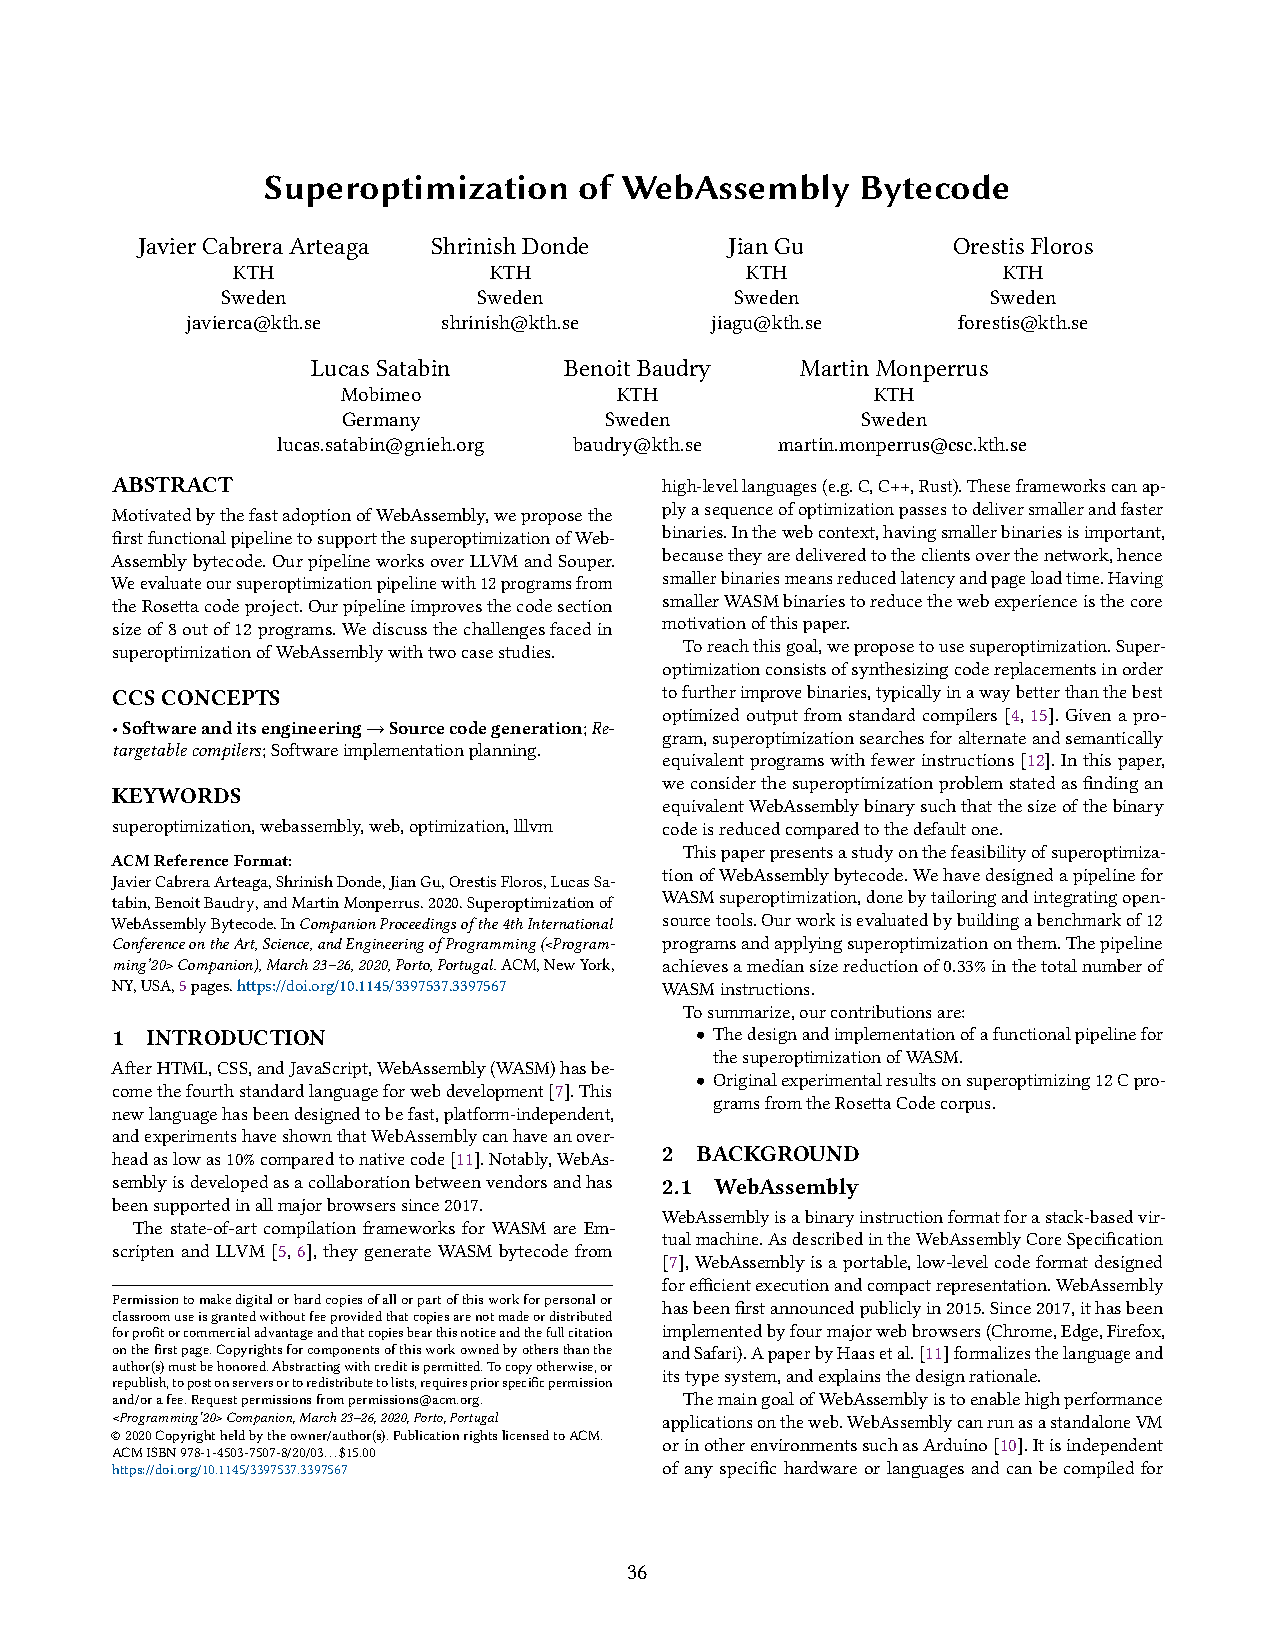
\includepdf[pages=1-5]{papers/souper.pdf}} % 
    {} %

% Add paper here
\chapter{CROW: Code Diversification for WebAssembly}

\textbf{Javier Cabrera-Arteaga}, Orestis Floros, Oscar Vera-Pérez, Benoit Baudry, Martin Monperrus\\
\emph{NDSS 2021, MADWeb}\\

\ifthenelse{\equal{\ADDCONTRIB}{True}}%
    {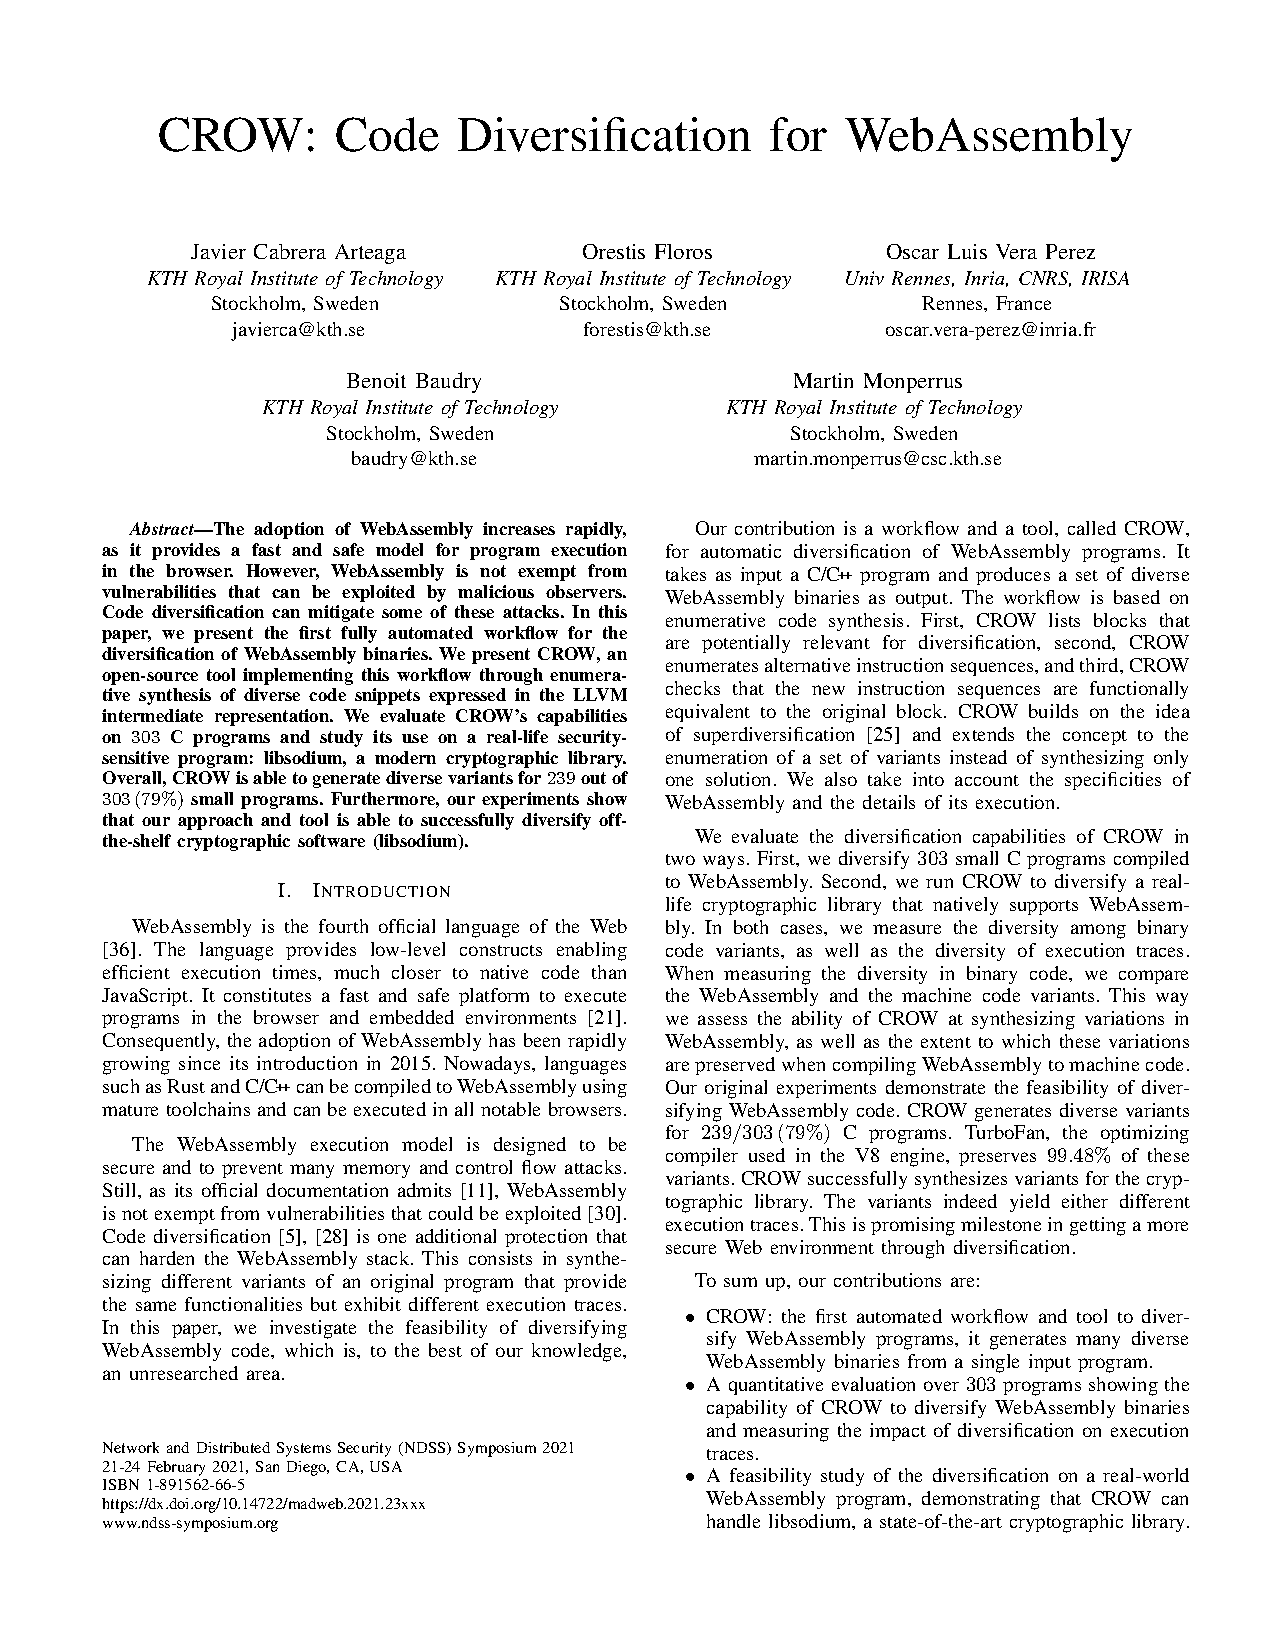
\includepdf[pages=1-12]{papers/crow.pdf}} %
    {} % 
    
\chapter{Multi-Variant Execution at the Edge}

\textbf{Javier Cabrera-Arteaga}, Pierre Laperdrix, Martin Monperrus, Benoit Baudry\\
\emph{Under review}\\

\ifthenelse{\equal{\ADDCONTRIB}{True}}%
    {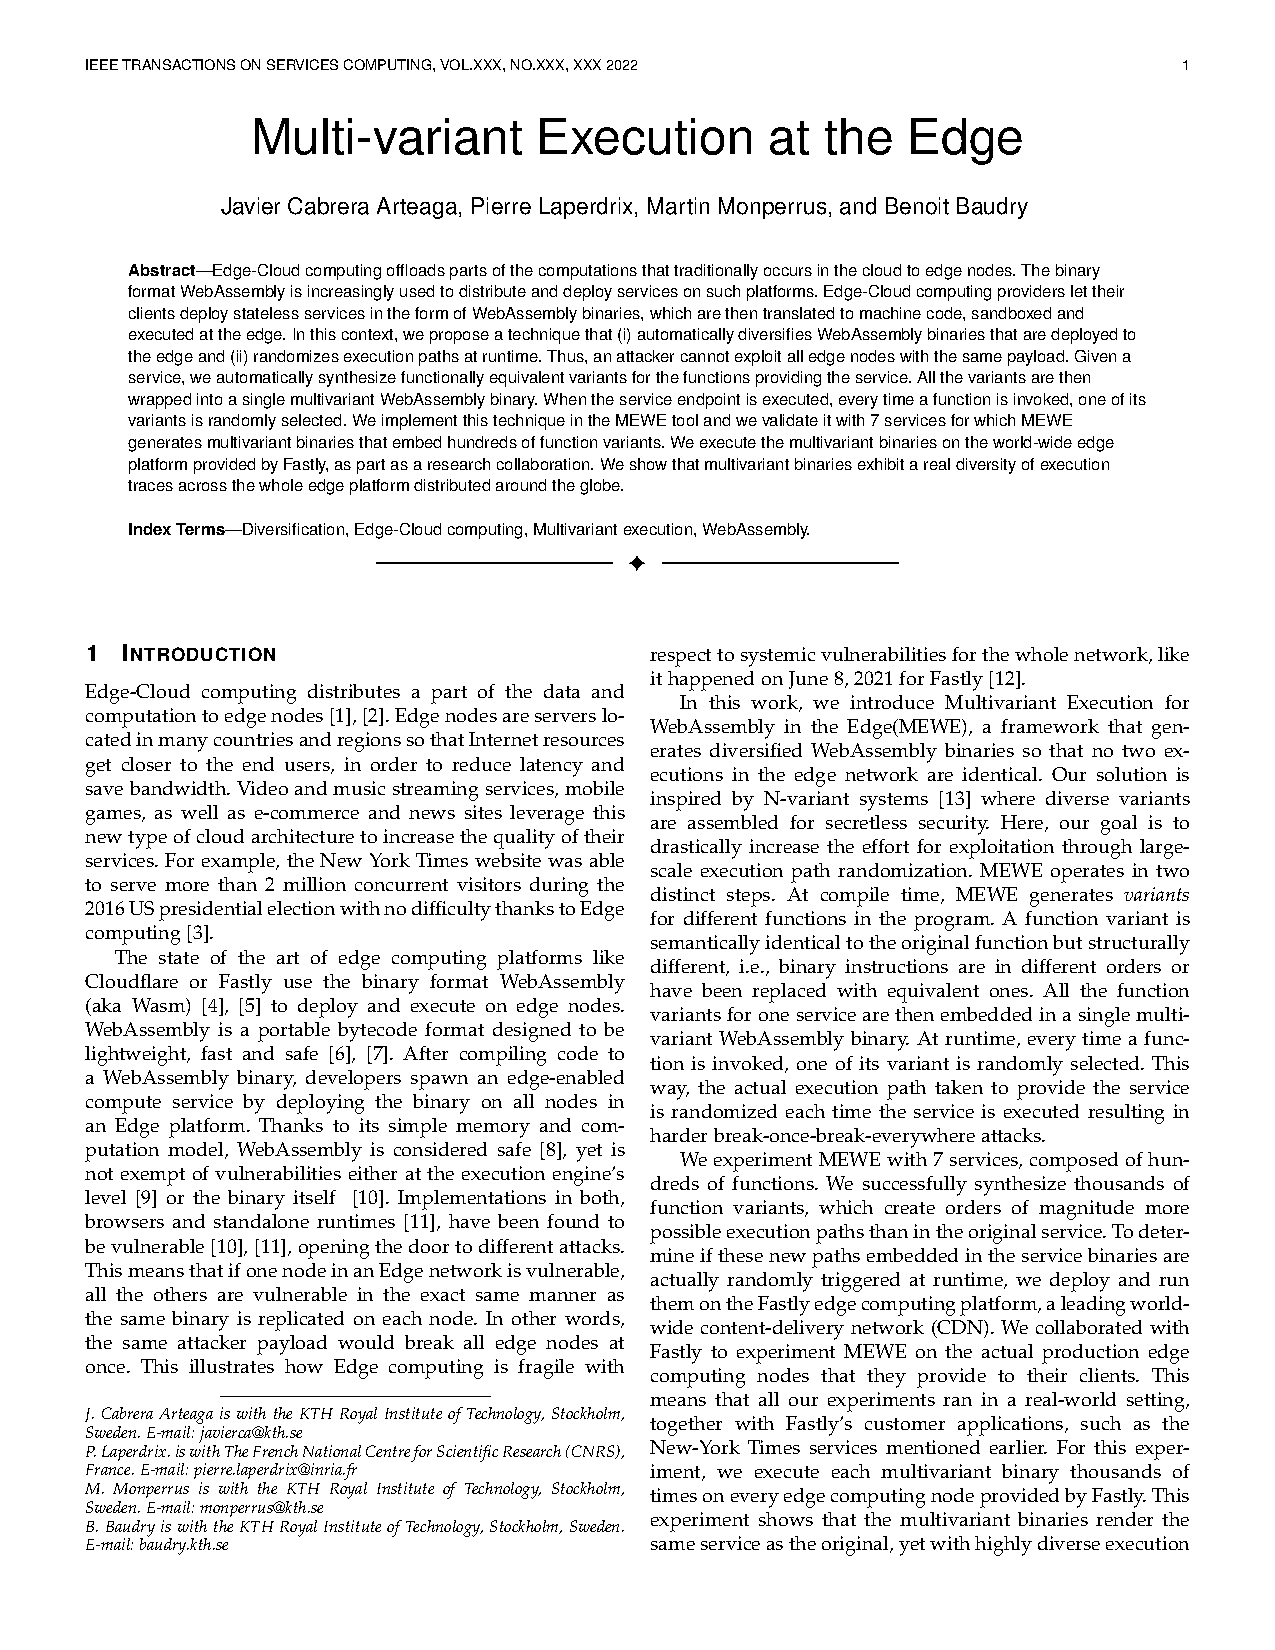
\includepdf[pages=1-12]{papers/mewe2.pdf}} %
    {} %
    
\chapter{Scalable Comparison of JavaScript V8 Bytecode Traces}

\textbf{Javier Cabrera-Arteaga}, Martin Monperrus, Benoit Baudry\\
\emph{SPLASH 2019, VMIL}\\


\ifthenelse{\equal{\ADDCONTRIB}{True}}%
    {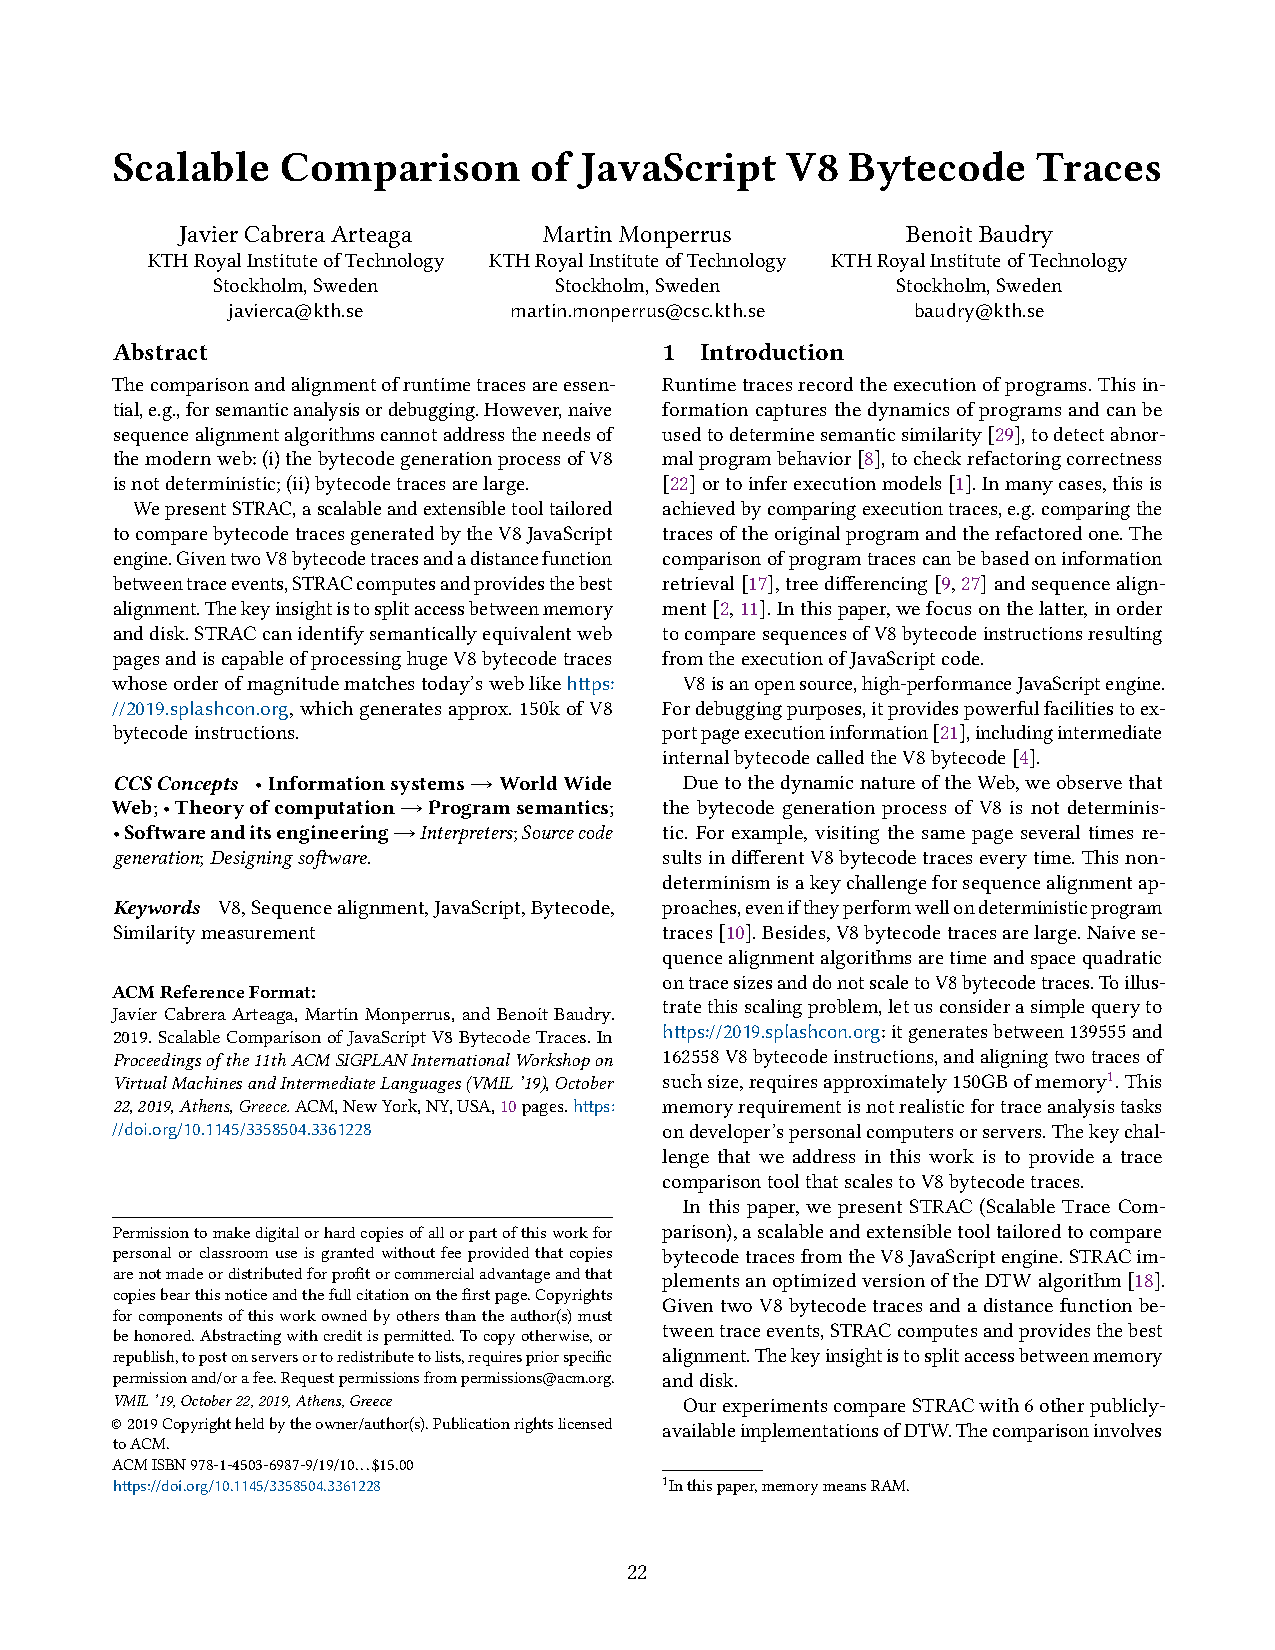
\includepdf[pages=1-10]{papers/STRAC.pdf}} %
    {} %
    

\printindex 

\end{document}
\endinput

